% simple.tex

\documentclass{article}[12pt,a4paper]

\usepackage{hyperref}
\hypersetup{
    colorlinks,
    citecolor=black,
    filecolor=black,
    linkcolor=black,
    urlcolor=black
}

\usepackage{tikz}
\usetikzlibrary{shapes.geometric, arrows}

\tikzstyle{startstop} = [rectangle, rounded corners, minimum width=3cm, minimum height=1cm,text centered, draw=black, fill=red!30]
\tikzstyle{io} = [trapezium, trapezium left angle=70, trapezium right angle=110, minimum width=3cm, minimum height=1cm, text centered, draw=black, fill=blue!30]
\tikzstyle{process} = [rectangle, minimum width=3cm, minimum height=1cm, text centered, text width=3cm, draw=black, fill=orange!30]
\tikzstyle{decision} = [diamond, minimum width=3cm, minimum height=1cm, text centered, draw=black, fill=green!30]
\tikzstyle{arrow} = [thick,->,>=stealth]

\usepackage{listings}
\usepackage{color}
\usepackage{graphicx}
\usepackage{longtable}
\usepackage{tikz-qtree}

\graphicspath{ {images/} }

\definecolor{codegreen}{rgb}{0,0.6,0}
\definecolor{codegray}{rgb}{0.5,0.5,0.5}
\definecolor{codepurple}{rgb}{0.58,0,0.82}
\definecolor{backcolour}{rgb}{0.95,0.95,0.92}
\definecolor{uigreen}{RGB}{82,170,94}
\definecolor{uiyellow}{RGB}{240,173,78}
\definecolor{uiblue}{RGB}{91,192,222}

\definecolor{lightgray}{rgb}{.9,.9,.9}
\definecolor{darkgray}{rgb}{.4,.4,.4}
\definecolor{purple}{rgb}{0.65, 0.12, 0.82}

\lstdefinelanguage{JavaScript}{
  keywords={typeof, new, true, false, catch, function, return, null, catch, switch, var, if, in, while, do, else, case, break},
  keywordstyle=\color{blue}\bfseries,
  ndkeywords={class, export, boolean, throw, implements, import, this},
  ndkeywordstyle=\color{darkgray}\bfseries,
  identifierstyle=\color{black},
  sensitive=false,
  comment=[l]{//},
  morecomment=[s]{/*}{*/},
  commentstyle=\color{purple}\ttfamily,
  stringstyle=\color{red}\ttfamily,
  morestring=[b]',
  morestring=[b]"
}

\lstset{
   language=JavaScript,
   backgroundcolor=\color{lightgray},
   extendedchars=true,
   basicstyle=\footnotesize\ttfamily,
   showstringspaces=false,
   showspaces=false,
   numbers=left,
   numberstyle=\footnotesize,
   numbersep=9pt,
   tabsize=2,
   breaklines=true,
   showtabs=false,
   captionpos=b
}

\lstdefinestyle{python}{
    backgroundcolor=\color{backcolour},   
    commentstyle=\color{codegreen},
    keywordstyle=\color{magenta},
    numberstyle=\tiny\color{codegray},
    stringstyle=\color{codepurple},
    basicstyle=\footnotesize,
    breakatwhitespace=false,         
    breaklines=true,                 
    captionpos=b,                    
    keepspaces=true,                 
    numbers=left,                    
    numbersep=5pt,                  
    showspaces=false,                
    showstringspaces=false,
    showtabs=false,                  
    tabsize=2
}

\begin{document}

\title{WJEC GCE Computing CG2 - Extended Task}

\author{Candidate Name: Daniel Roberts\\
        Candidate Number: 4699\\
        Centre Name: Shrewsbury Sixth Form College\\
        Centre Number: 29285}

\date{}

\maketitle

\tableofcontents

\cleardoublepage

\part{Analysis and Design}
This part of documentation contains analysis that was performed on Parkwood Vale Harriers, taking into account what running club asked for in their brief, and exploring these requirements. It also covers preliminary design that was created for system, including interface design for every page, design of data structures and process design, detailing different algorithms that have been used, and how system interacts with itself.

\section{Problem Definition}
\subsection{Background}
Parkwood Vale Harriers is a running club that serves fitness needs of many different members, through regular sessions, as well as races. club gets involved in local community, a position that consists, in part, of raising money for local charities. 

Recently, club has decided to raise money for one of charities by putting on a relay event, wherein a team of runners will run, non-stop, from John O\textsc{\char13} Groats to Land’s End, in shortest time possible. team will consist of eight members, and each runner will run for an hour at a time, whilst others rest in minibus. entire trip is estimated to take three days and as a result of this, each member of team will have to be very fit.

In order to increase their chances of completing run, club has decided to find out most appropriate team, based on results of a physically challenging programme. This programme will consist of running, cycling and swimming, and will serve to ensure that only top members of club are included in team.

\subsection{Broad Aims}
running club has commissioned  a computer based system that will allow runners to keep an accurate record of their running, cycling and swimming sessions. This data will then be used to calculate an informed decision of most appropriate team for relay race.

The system must allow each runner to monitor their progress during programme, clearly showing them extent to which they have improved. As such, the system must provide an interface to allow runner to add each session they perform, with spaces for type of training, time spent, how hard they pushed themselves, and other such parameters. Using this data, the system must then calculate number of calories burned in session, providing a series of data points through which performance of runner can be monitored.

To further aid in this, the system must be able to output these sessions in a clear format that runner is able to clearly understand. This can be achieved through use of tables to display each session in a listed, tabular format, as well as through graphs and charts to display data in a graphical form; this maes overall performance trends easy to visualise.

Due to nature of the system, ability to store certain personal information, such as name, age and weight of runner, must also be included. runner should have ability to input this information themselves, most likely upon first use of the system. There should be ability to modify this data, in result of an error being made or circumstances of runner changing.

An important aspect of the system, and one that is key to promoting competitive values of club, is ability to compare results with other participants in program. This area of the system should allow runners to compare key aspects of their performance, such as results of their individual sessions, as well as their overall performance over time in all three of activities.

As the main point of the system, ability to select final team must also be included. By analysing data points provided by runners, the system should be able to choose most appropriate team.

\subsection{Limitations}
Though brief provided by running club contains several good ideas and acts as an effective base upon which to work, there are a number of areas which running club has not thought about that could be factored into solution, creating a more effective system. 

One very important factor that running club has left out is security. In a system like this, where intensely personal data is being stored, including data that user may not which to become public, such as their weight, it is important that data is stored in a secure manner that allows only those with correct permissions to access it. 

Another issue with brief is that of an objective decision being made when selecting team. Running a marathon is about far more than just physical fitness; more personal aspects, such as how well runners get along and different roles within team, should also be taken into account for maximum efficiency. The system would be unable to do this (without each runner giving their opinion on others, which is unrealistic), and so team it comes up with may not be most appropriate choice. 

Another limitation in the system is that data will have to be entered manually: there is no way of taking data from some sort of personal tracking device. This could result in some issues with accuracy, or even with malpractice: people entering exaggerated data in order to manipulate rankings and make themselves seem better. A mixture of validation and verification can be put in place to prevent this, such as ensuring users cannot go for a straight eight hour swim (something which is obviously unrealistic), but this will be unable to catch all cases of exaggeration; it is therefore necessary to rely on goodwill and sportsmanship of runners.

Furthermore, the system relies on premise that runners will add every session they perform to application. It is not unlikely that they will go on unsolicited sessions that they do not bother adding, or they may simply forget. There is no foolproof manner to prevent these occurences, but a number of steps can be taken to reduce their likelihood, such as by making process of adding a session as simple as possible - easier process is, more likely runner is to do it.

In addition, the brief asks for only top eight members of running team to be calculated. This does not take into account possibilities of injuries or runners dropping out for other reasons; as such, the system should also calculate a number of reserve runners, in event of an accident.

\subsection{Assumptions}
Throughout the system, a number of assumptions have been made in order to increase ease of development. 

One of these is that in each individual session, only one method of exercise will be used, such as breaststroke for an entire swimming session or a leisurely speed for an entire cycling session. Though this is alleviated to some extent by ability to add multiple sessions for each sport on a single day, assumption still has to be made. 

In addition to this, assumption that each session lasts for at least an hour has been made: time picker only uses stages of sixty minutes, as opposed to thirty or fifteen.

Naturally, the system also assumes that user is relatively proficient with a computer based interface. Effort has been put in to make the system as user friendly and as easy to use as possible, but someone using a computer for first time will undoubtedly find it more difficult than someone with at least a little experience.

\subsection{Objectives}
In order for the system to be of an acceptable quality, a number of objectives will have to be fulfilled. The system must:

\begin{itemize}
    \item Have a simple, clear interface that allows tasks to be performed easily.
    \item Allow runner to add, view, update and, if they choose, delete their personal information, such as their name, email address, date of birth and phone number.
    \item Allow runner to add, view and delete sessions they perform in over course of period; this will include information like date and time of session, speed they were at, and how well it went.
    \item Persistently store this data in appropriately named tables in a database.
    \item Ensure security of this data by giving each runner their own personal account, protected by a username and an encrypted password.
    \item Calculate thenumber of calories burned in each session, by taking into account runner's weight, time spent on session, nature of session, and how well the runner thought it went.
    \item Allow user to view graphical, interactive graphs of their sessions, allowing them to easily view trends in their performance.
\end{itemize}

\subsection{Justification of Proposed Solution}
When building a solution to a problem like one faced by Parkwood Vale Harriers, there are generally two methods available: utilising features of an existing software package, such as Microsoft Office Access, or programming an existing solution in a programming language, such as Visual Basic or Python. Both have their advantages and drawbacks: by utilising an existing package, much of system will already be developed; it only remains to manipulate system to meet needs of brief; but, on other hand, one can be limited by restrictions of software package, perhaps preventing final solution being as capable as it might otherwise have been.

An original solution created using a programming language would suffer from rather opposite issues: as a result of practically endless results that can be achieved through their use, there is a definite learning curve that is not present (or is less exacerbated) in software packages; as a result of this, development time will likely be considerably longer. Despite these drawbacks, it is clear that, if a programming language is used, final solution is likely to be of a higher quality: not only can more advanced features be implemented, these features - as well as those of a more basic level - are likely to be of a higher quality.  In addition, developer will have a greater understanding of system, as they will have built it entirely themselves (aside from any additional packages/libraries used); this will aid in areas like debugging, and will also make it easier to write up system documentation and like.

The question then falls to exactly which programming language is most appropriate. There are a large number of languages available, ranging from \textit{compiled} languages like Java, C\# and Visual Basic to \textit{interpreted} languages like Ruby, Python and PHP. differences between compiled and iterpreted languages are complex and varied, but, in essence, compiled languages are likely to perform algorithms more quickly (due to directly using native code of target machine), whereas code written in an interpreted language can be executed ``on the fly'', so to speak, increasing development speed. 

\section{Data Structures and Methods of Access}
In order to persistently store runner's data, a database is needed. As is custom with applications of this sort, there will be one single database file, within which will be a number of tables. system will also make use of a number of arrays and JSON structures, to temporarily store data.

\subsection{Database Tables}
The system will use SQLite database system. SQLite is a very popular database system (in same vein as MySQL). All of the database tables will be accessed sequentially - every item is ordered according to their primary key, which, as is custom for an SQLite database, is always an id number stored as an integer.
\\\\\textbf{\textit{A note on validation: }}\textit{SQLite does not perform any validation itself. All validation will be performed during processing of data, before it is added into database. As such, details on validation performed on data saved to these tables can be found in their relevant section.}

\subsubsection{Users Table}
This table will store personal information for each runner. Whenever a runner creates an account, the data they input into registration form will end up in this table.

\begin{table}[htbp]
\begin{tabular}{|l|l|l|l|l|}
\hline
\textbf{Field Name}     & \textbf{Primary Key} & \textbf{Typical Data} & \textbf{Data Type} \\ \hline
id             & True        & 01                   & Integer   \\ \hline
name           & n/a         & John Smith           & String    \\ \hline
email          & n/a         & john@smith.com       & String    \\ \hline
username       & n/a         & john5                & String    \\ \hline
password\_hash & n/a         & pbkdf2:sha1:1000\$02 & String    \\ \hline
dob            & n/a         & 1997-02-02           & Date      \\ \hline
phone          & n/a         & 07722895880          & String    \\ \hline
weight         & n/a         & 74                   & Integer   \\ \hline
distance       & n/a         & less than 1          & String    \\ \hline
joined         & n/a         & 2015-01-04           & Date      \\ \hline
charity\_event & n/a         & True                 & Boolean   \\ \hline
\end{tabular}
\caption{Users Table}
\end{table}

Each user will be given an id which serves as their primary key; it is automatically incremented whenever a new user is added, hence the data type of integer. The name will be used as an identifier throughout the system; as a string of characters, it has been given the string data type. Likewise with the email field: it can contain a combination of letters, numbers and other characters, and so has been will be set as a string. The username field will be a combination of the runner's first name and a random number; as such it will be a string. The password hash field stores an encrypted version of the user's password; depending on the length of password, it can contain a very large number of letters, numbers and symbols - it is therefore a string. The dob field will store the runner's date of birth; the most appropriate data type would therefore be date; likewise with the date runner joined the application. No calculations are being performed on the runner's phone number, so it is more efficient to store it as a string - one character takes just 1 bit. Conversely, calculations will performed with runner's weight, so it is appropriate to store it as an integer. The charity event field stores either True or False depending on whether the runner wishes to be chosen to run in charity event; the most appropriate data type is therefore Boolean.

\subsubsection{Activities Table}

Every activity that runners add will be given its own record in this table. It is accessed sequentially, according to id of each activity. In addition, each activity will be linked to a user through a foreign key, called user\_id. It is a one-to-many relationship.

\begin{table}[h]
\begin{tabular}{|l|l|l|l|}
\hline
\textbf{Field Name} & \textbf{PK / FK} & \textbf{Typical Data} & \textbf{Data Type} \\ \hline
id                  & Primary          & 01                    & Integer            \\ \hline
sport               & n/a              & running               & String             \\ \hline
effigy              & n/a              & 5 mph                 & String             \\ \hline
date                & n/a              & 2015-01-04            & Date               \\ \hline
start               & n/a              & 8:00AM                & String             \\ \hline
finish              & n/a              & 10:00AM               & String             \\ \hline
hours               & n/a              & 2                     & Integer            \\ \hline
opinion             & n/a              & Brilliant             & String             \\ \hline
thoughts            & n/a              & It was great.         & String             \\ \hline
user\_id            & Foreign          & 02                    & Integer            \\ \hline
\end{tabular}
\caption{Activities Table}
\end{table}

id of each activity serves as its primary key; it is automatically incremented whenever a new activity is added, hence data type of integer. sport field will be a string; it will store type of sport that activity belongs to, and so string is most appropriate data type. effigy field will store specific detail for each activity, such as speed for running sessions, or type of stroke for swimming sessions. Due to wide range of options that can be stored in this, and fact that no calculations will be performed, string data type would be most appropriate. 

\section{User Interface Design}
The system will use a web based, graphical user interface. It will be simple and easy to use, making use of user interface paradigms well known to users, such as buttons, form inputs and drop-down boxes, through their use of other computer systems. In order to increase usability, the system will make use of a consistent colour palette - each sport will be associated with a particular colour:
\\\\\textcolor{uigreen}{Green - rgb(82, 170, 94) - associated with running}
\\\textcolor{uiyellow}{Yellow - rgb(240, 173, 78) - associated with cycling}
\\\textcolor{uiblue}{Blue - rgb(91, 192, 222) - associated with swimming}
\\\\In addition, the system will make use of a consistent font: Raleway, and its variants. Raleway is a distinctive yet readable sans-serif font, and is only font used throughout system. It can be seen in the user interface documentation.

\subsection{Main Layout Template}
To ensure visual consistency throughout the system, every page will derive itself from a master template, which will contain aspects like navigation, footer and placement of elements.

\begin{figure}[h!]
  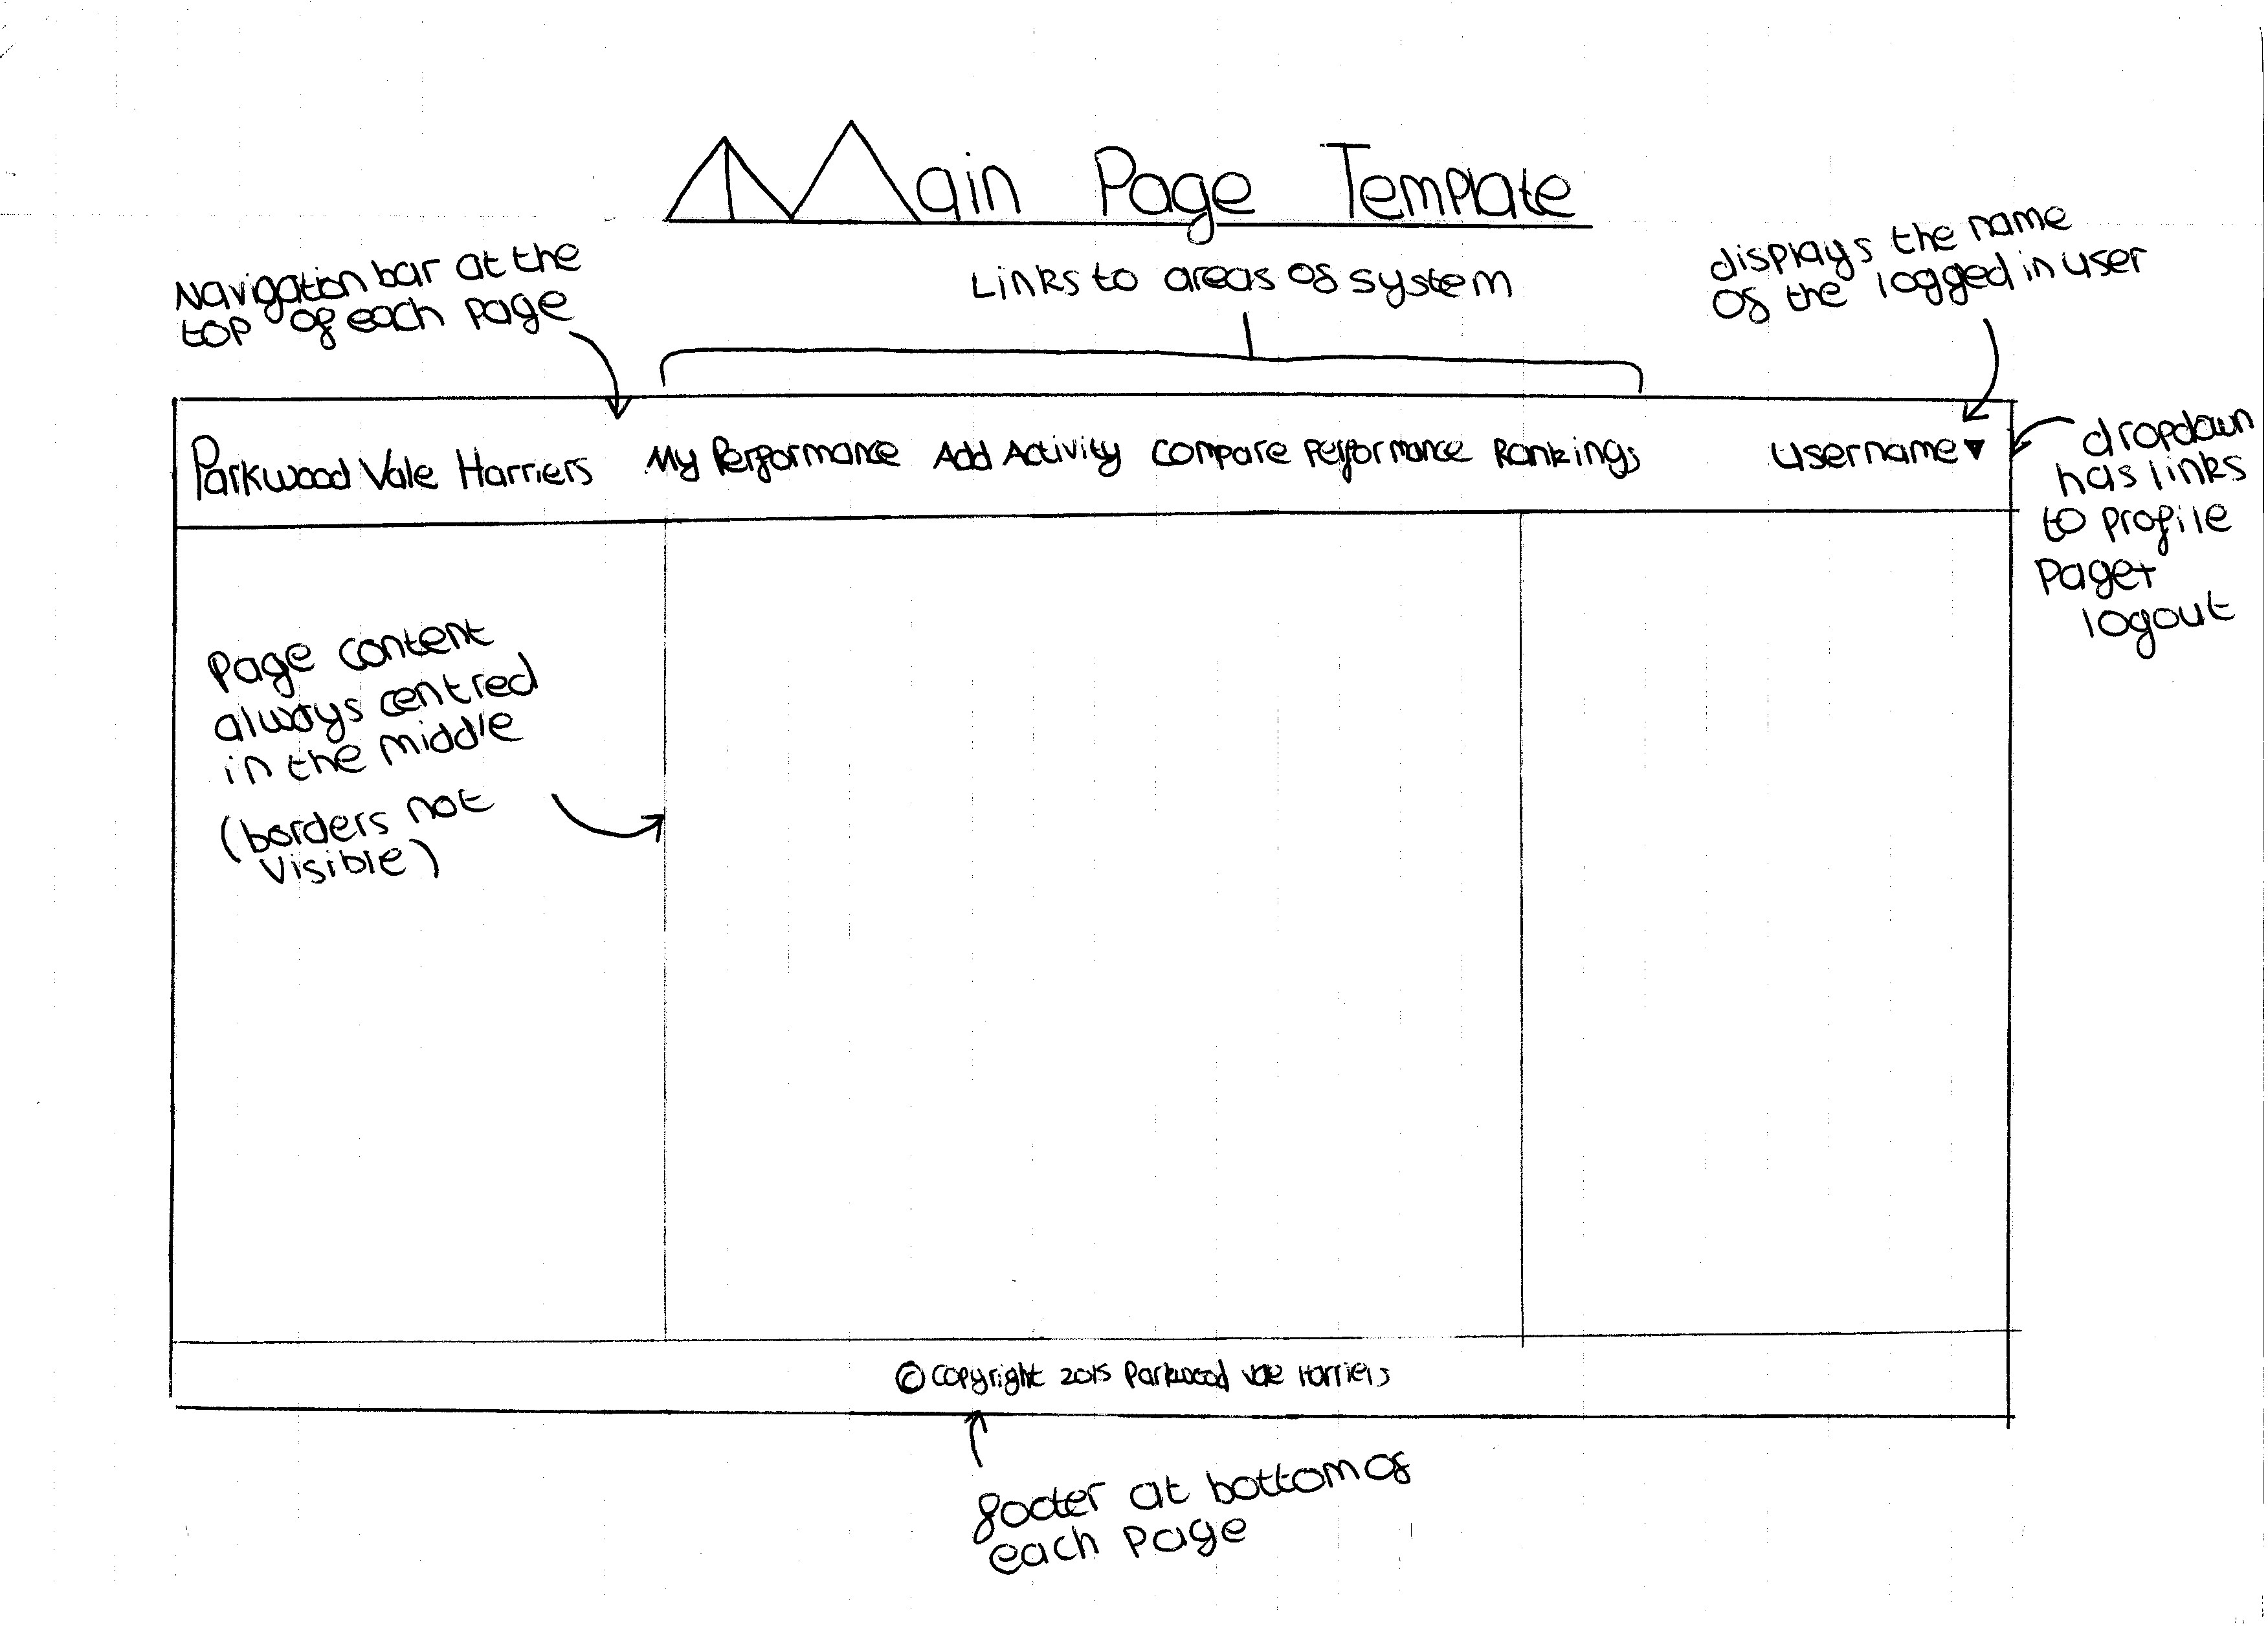
\includegraphics[scale=0.45]{design_ui/layout}
\end{figure}
\clearpage

\subsection{Register Page}
\begin{figure}[h!]
  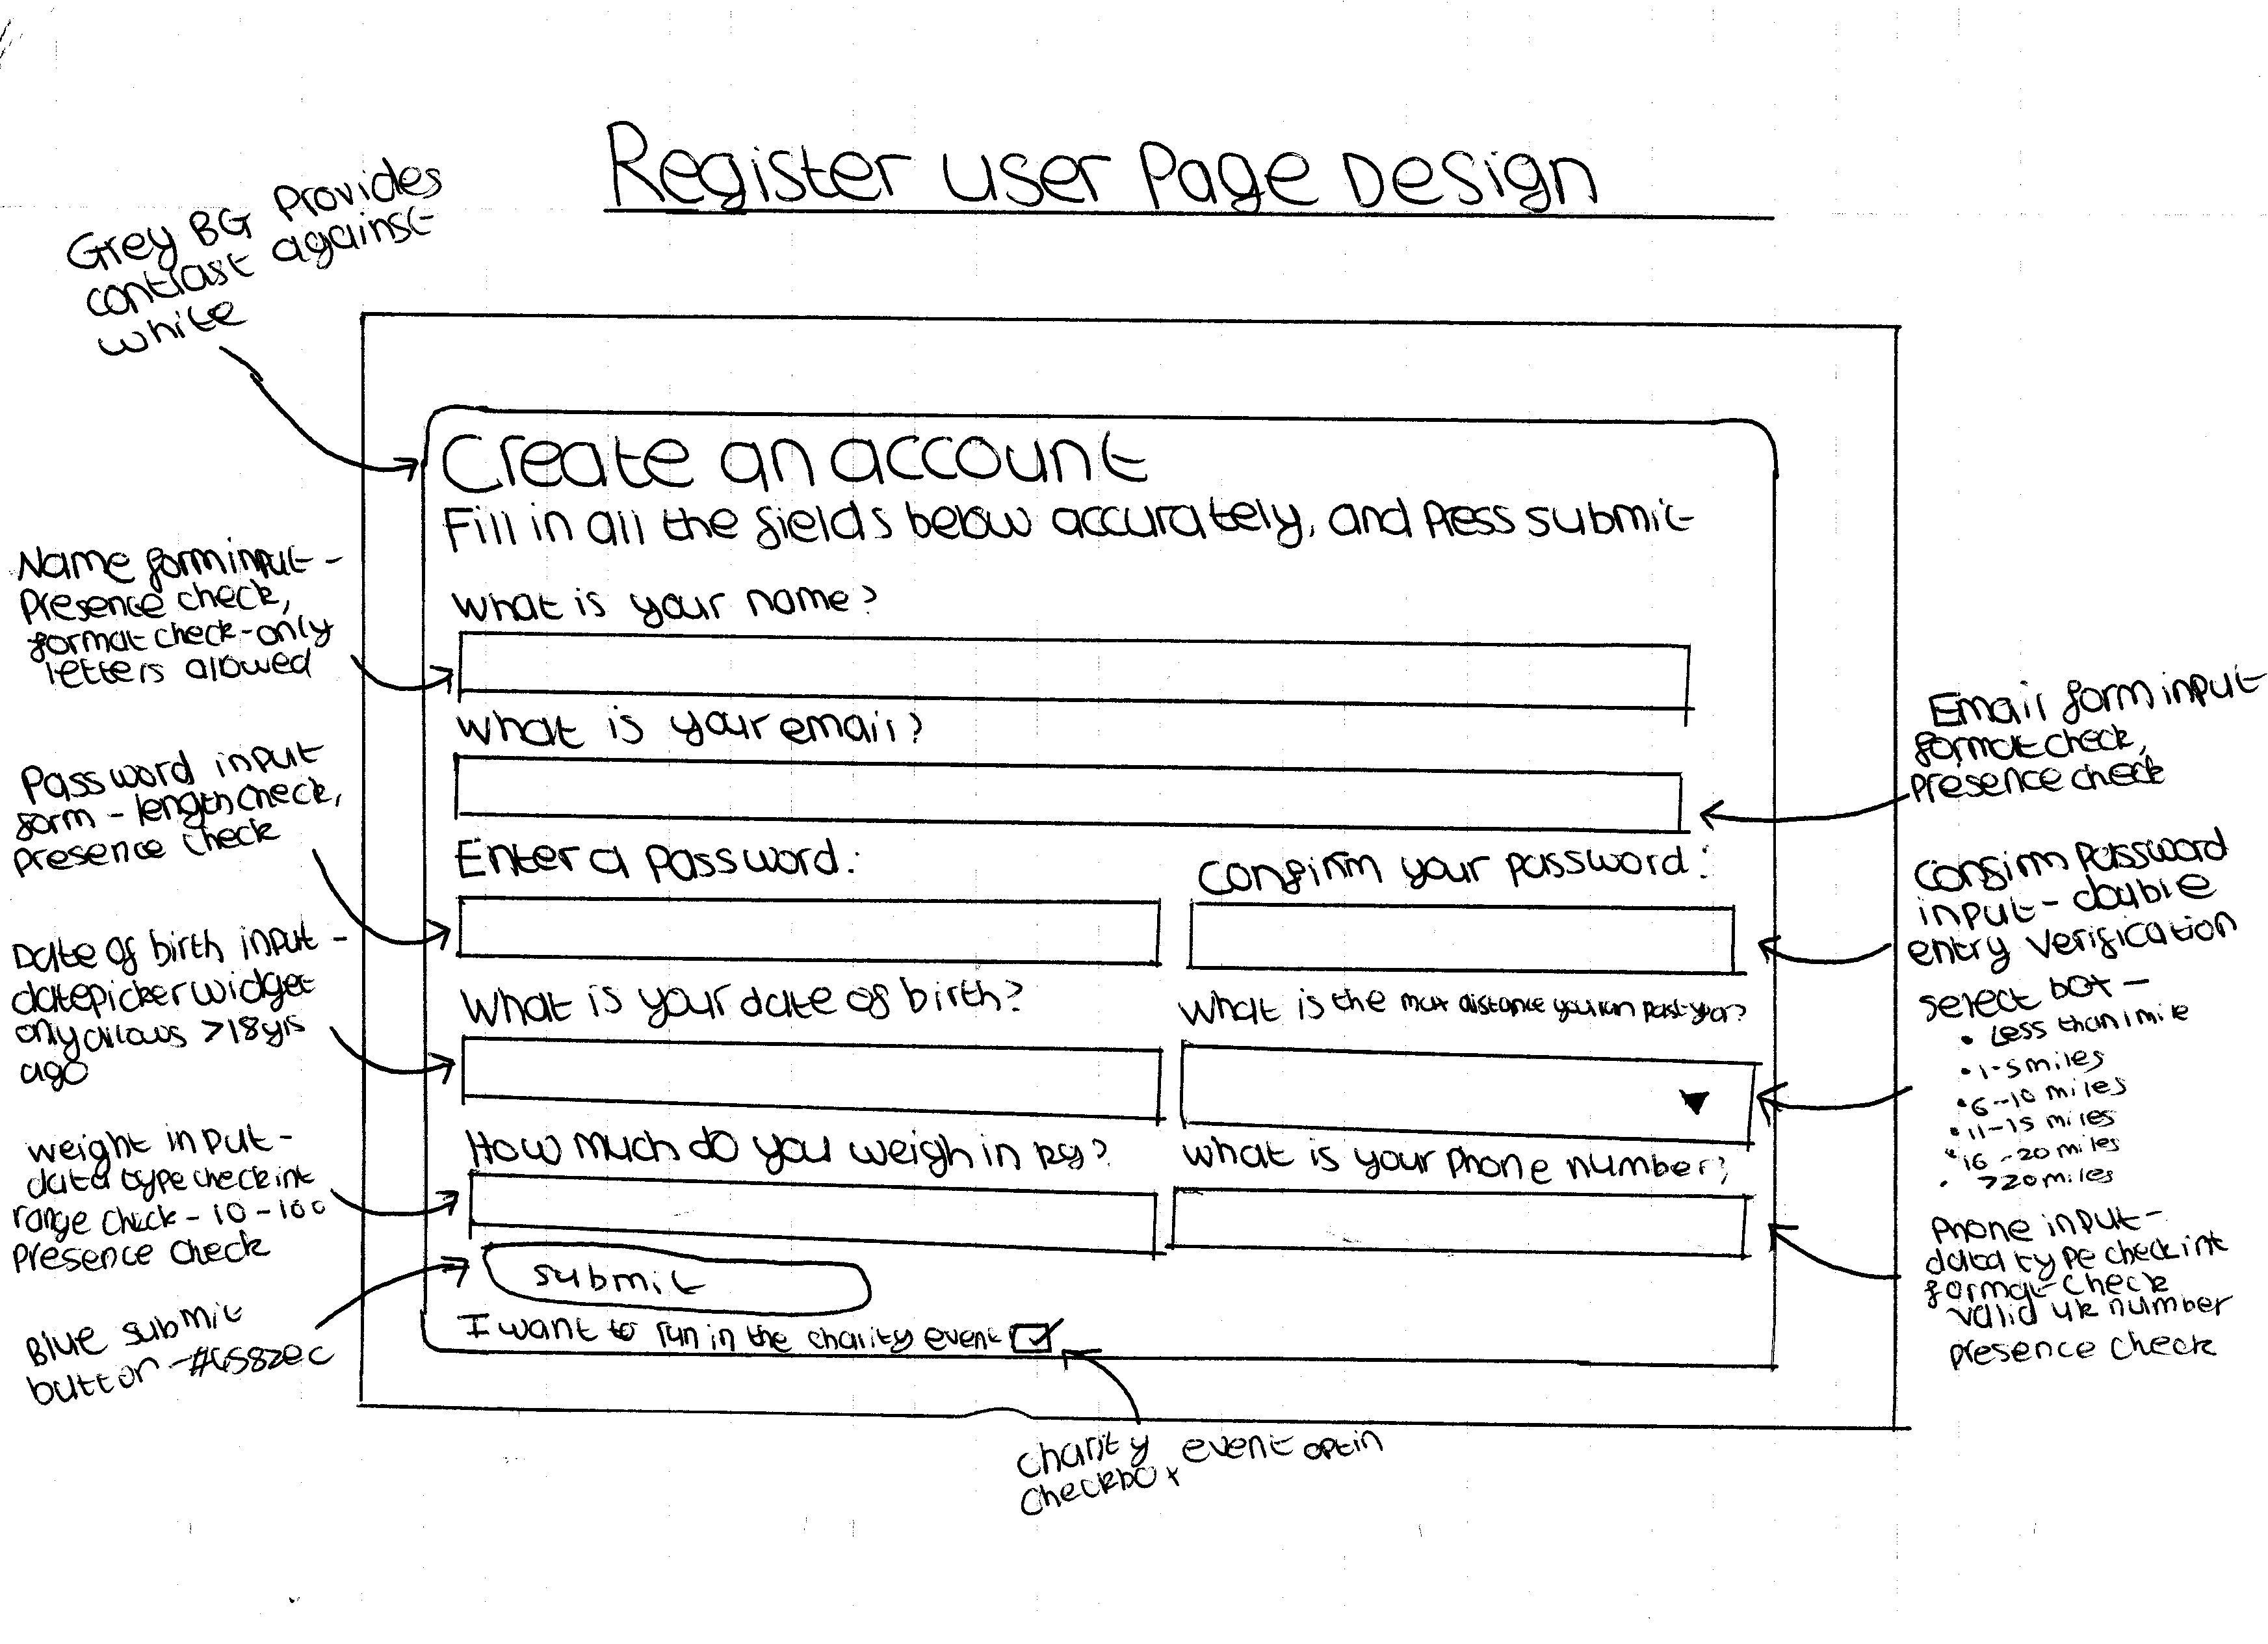
\includegraphics[scale=0.55]{design_ui/register}
\end{figure}
\clearpage

\subsection{Login Page}
\begin{figure}[h!]
  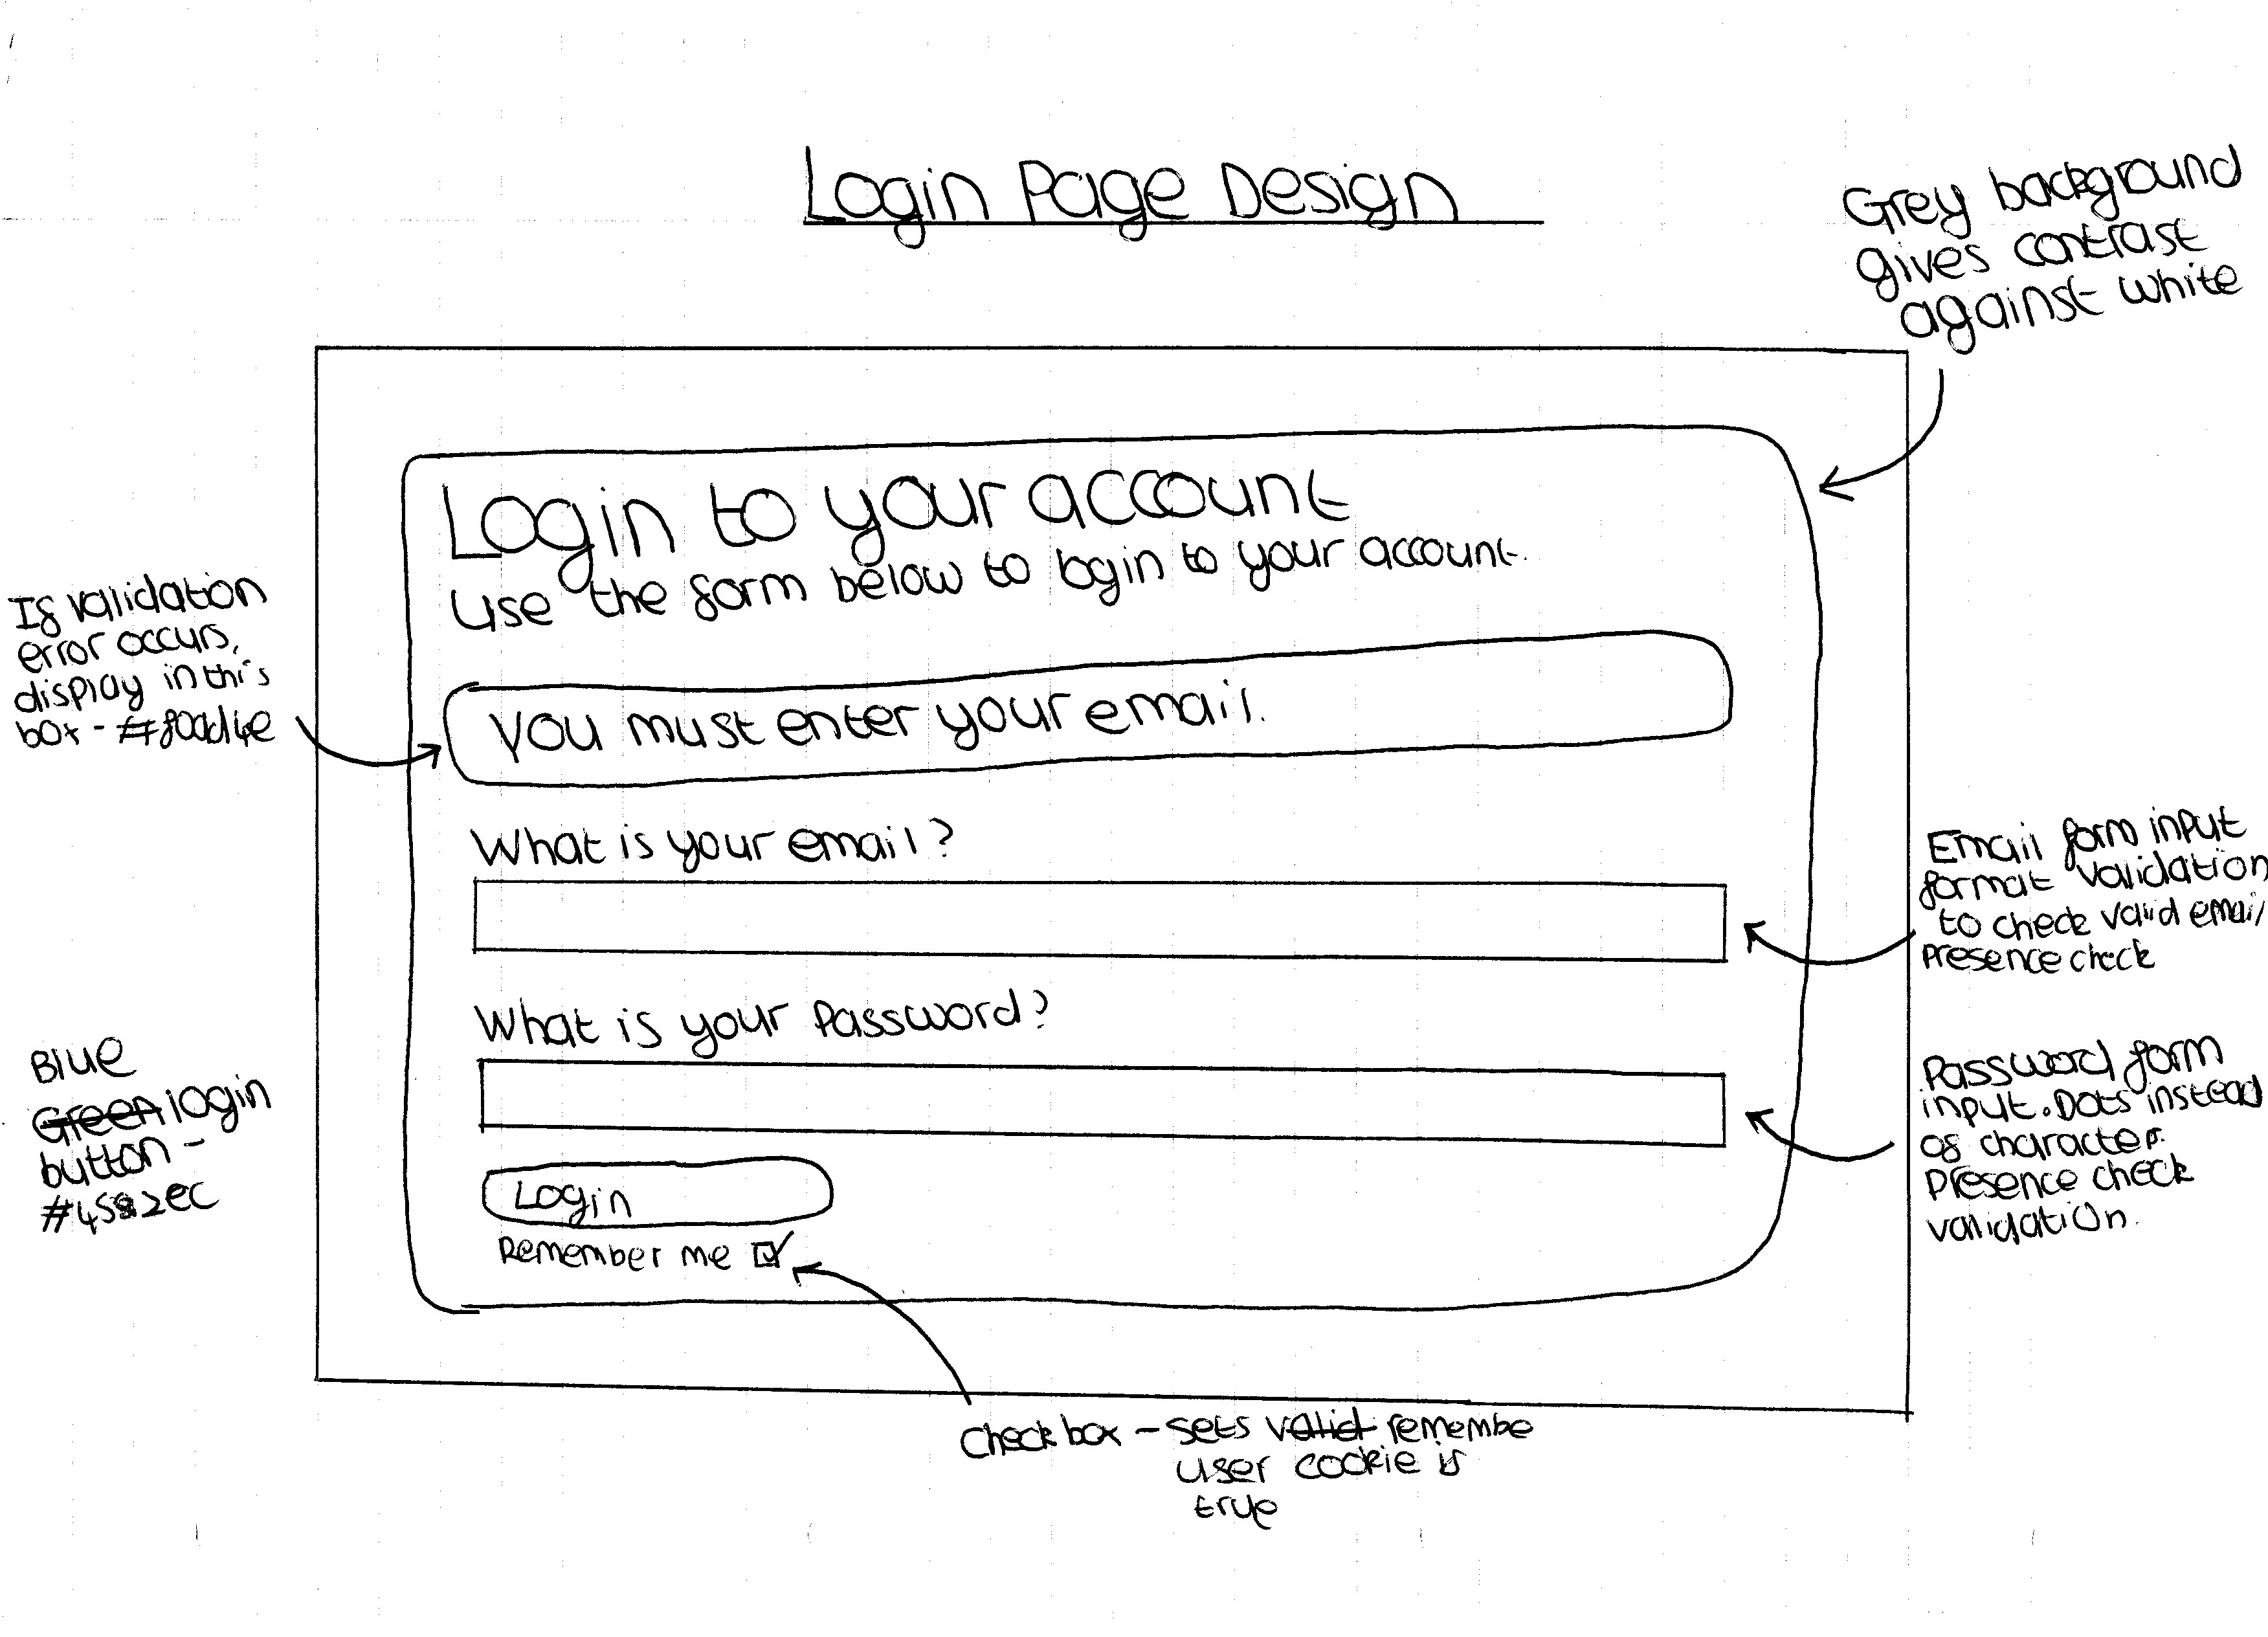
\includegraphics[scale=0.55]{design_ui/login}
\end{figure}
\clearpage

\subsection{Performance Page}
To ensure visual consistency throughout the system, every page will derive itself from a master template, which will contain aspects like navigation, footer and placement of elements.

\begin{figure}[h!]
  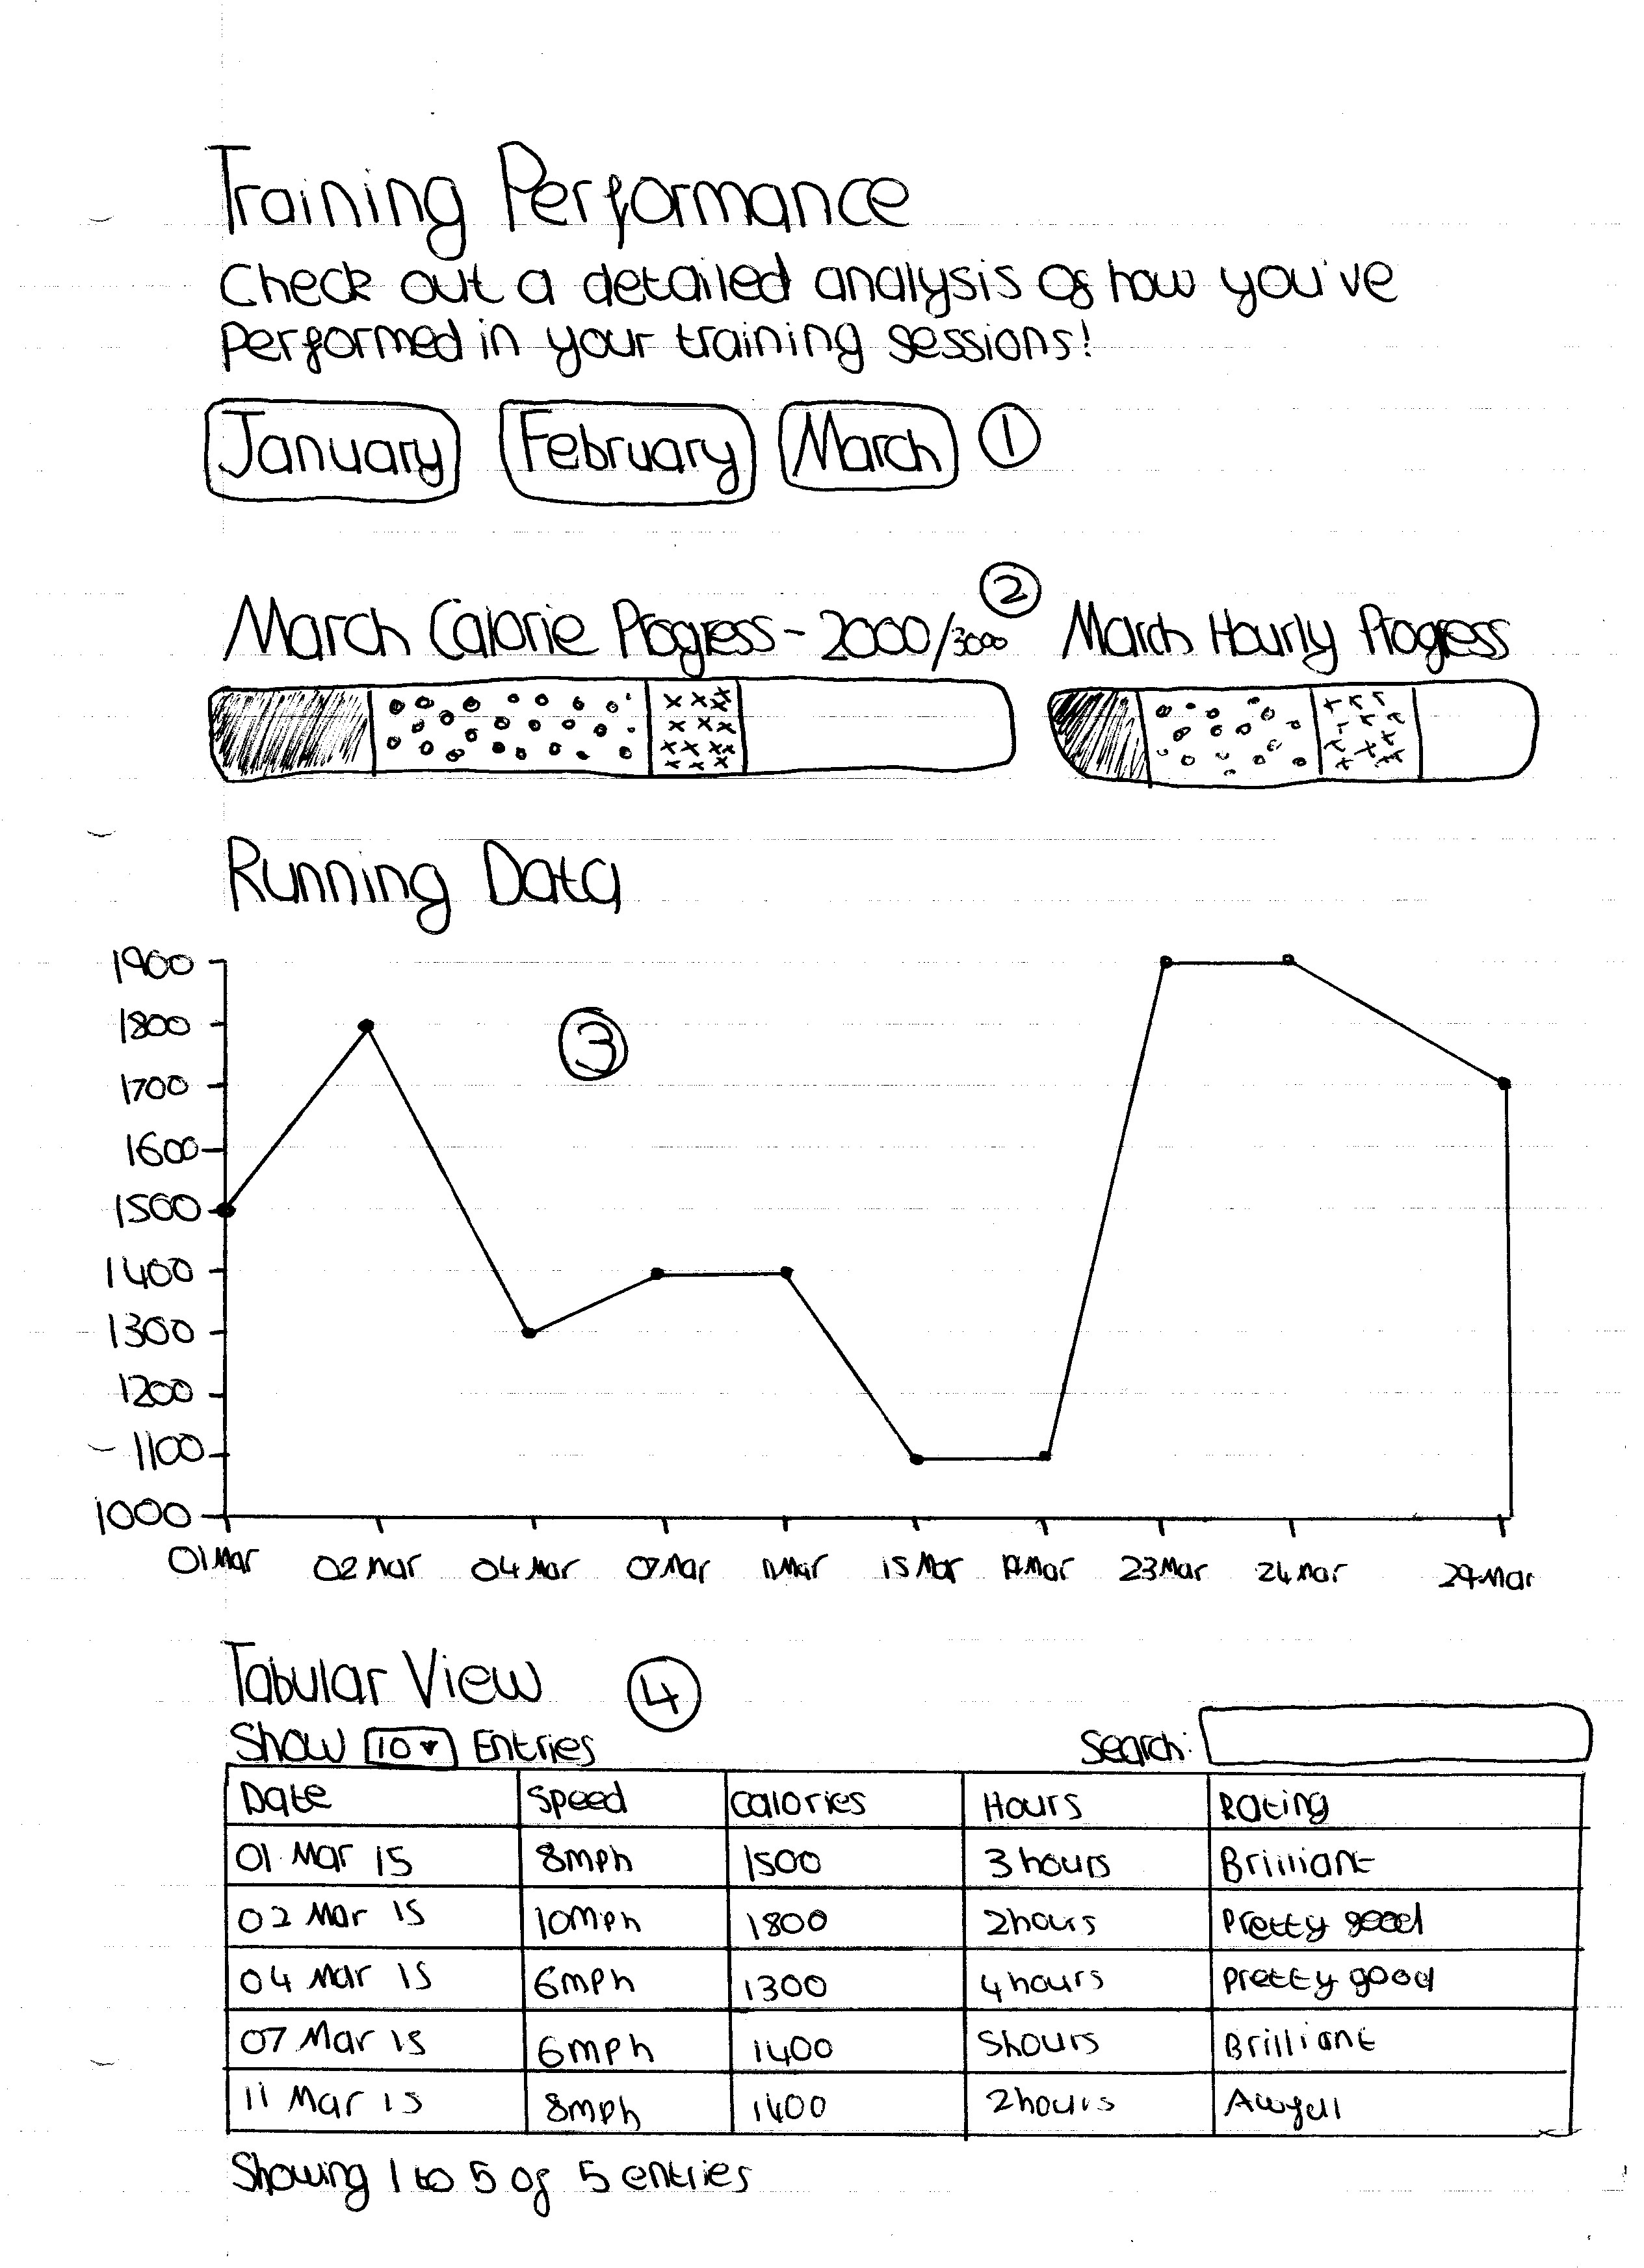
\includegraphics[scale=0.55]{design_ui/user_performance}
\end{figure}
\clearpage

\subsection{Add Training Page}
To ensure visual consistency throughout the system, every page will derive itself from a master template, which will contain aspects like navigation, footer and placement of elements.

\begin{figure}[h!]
  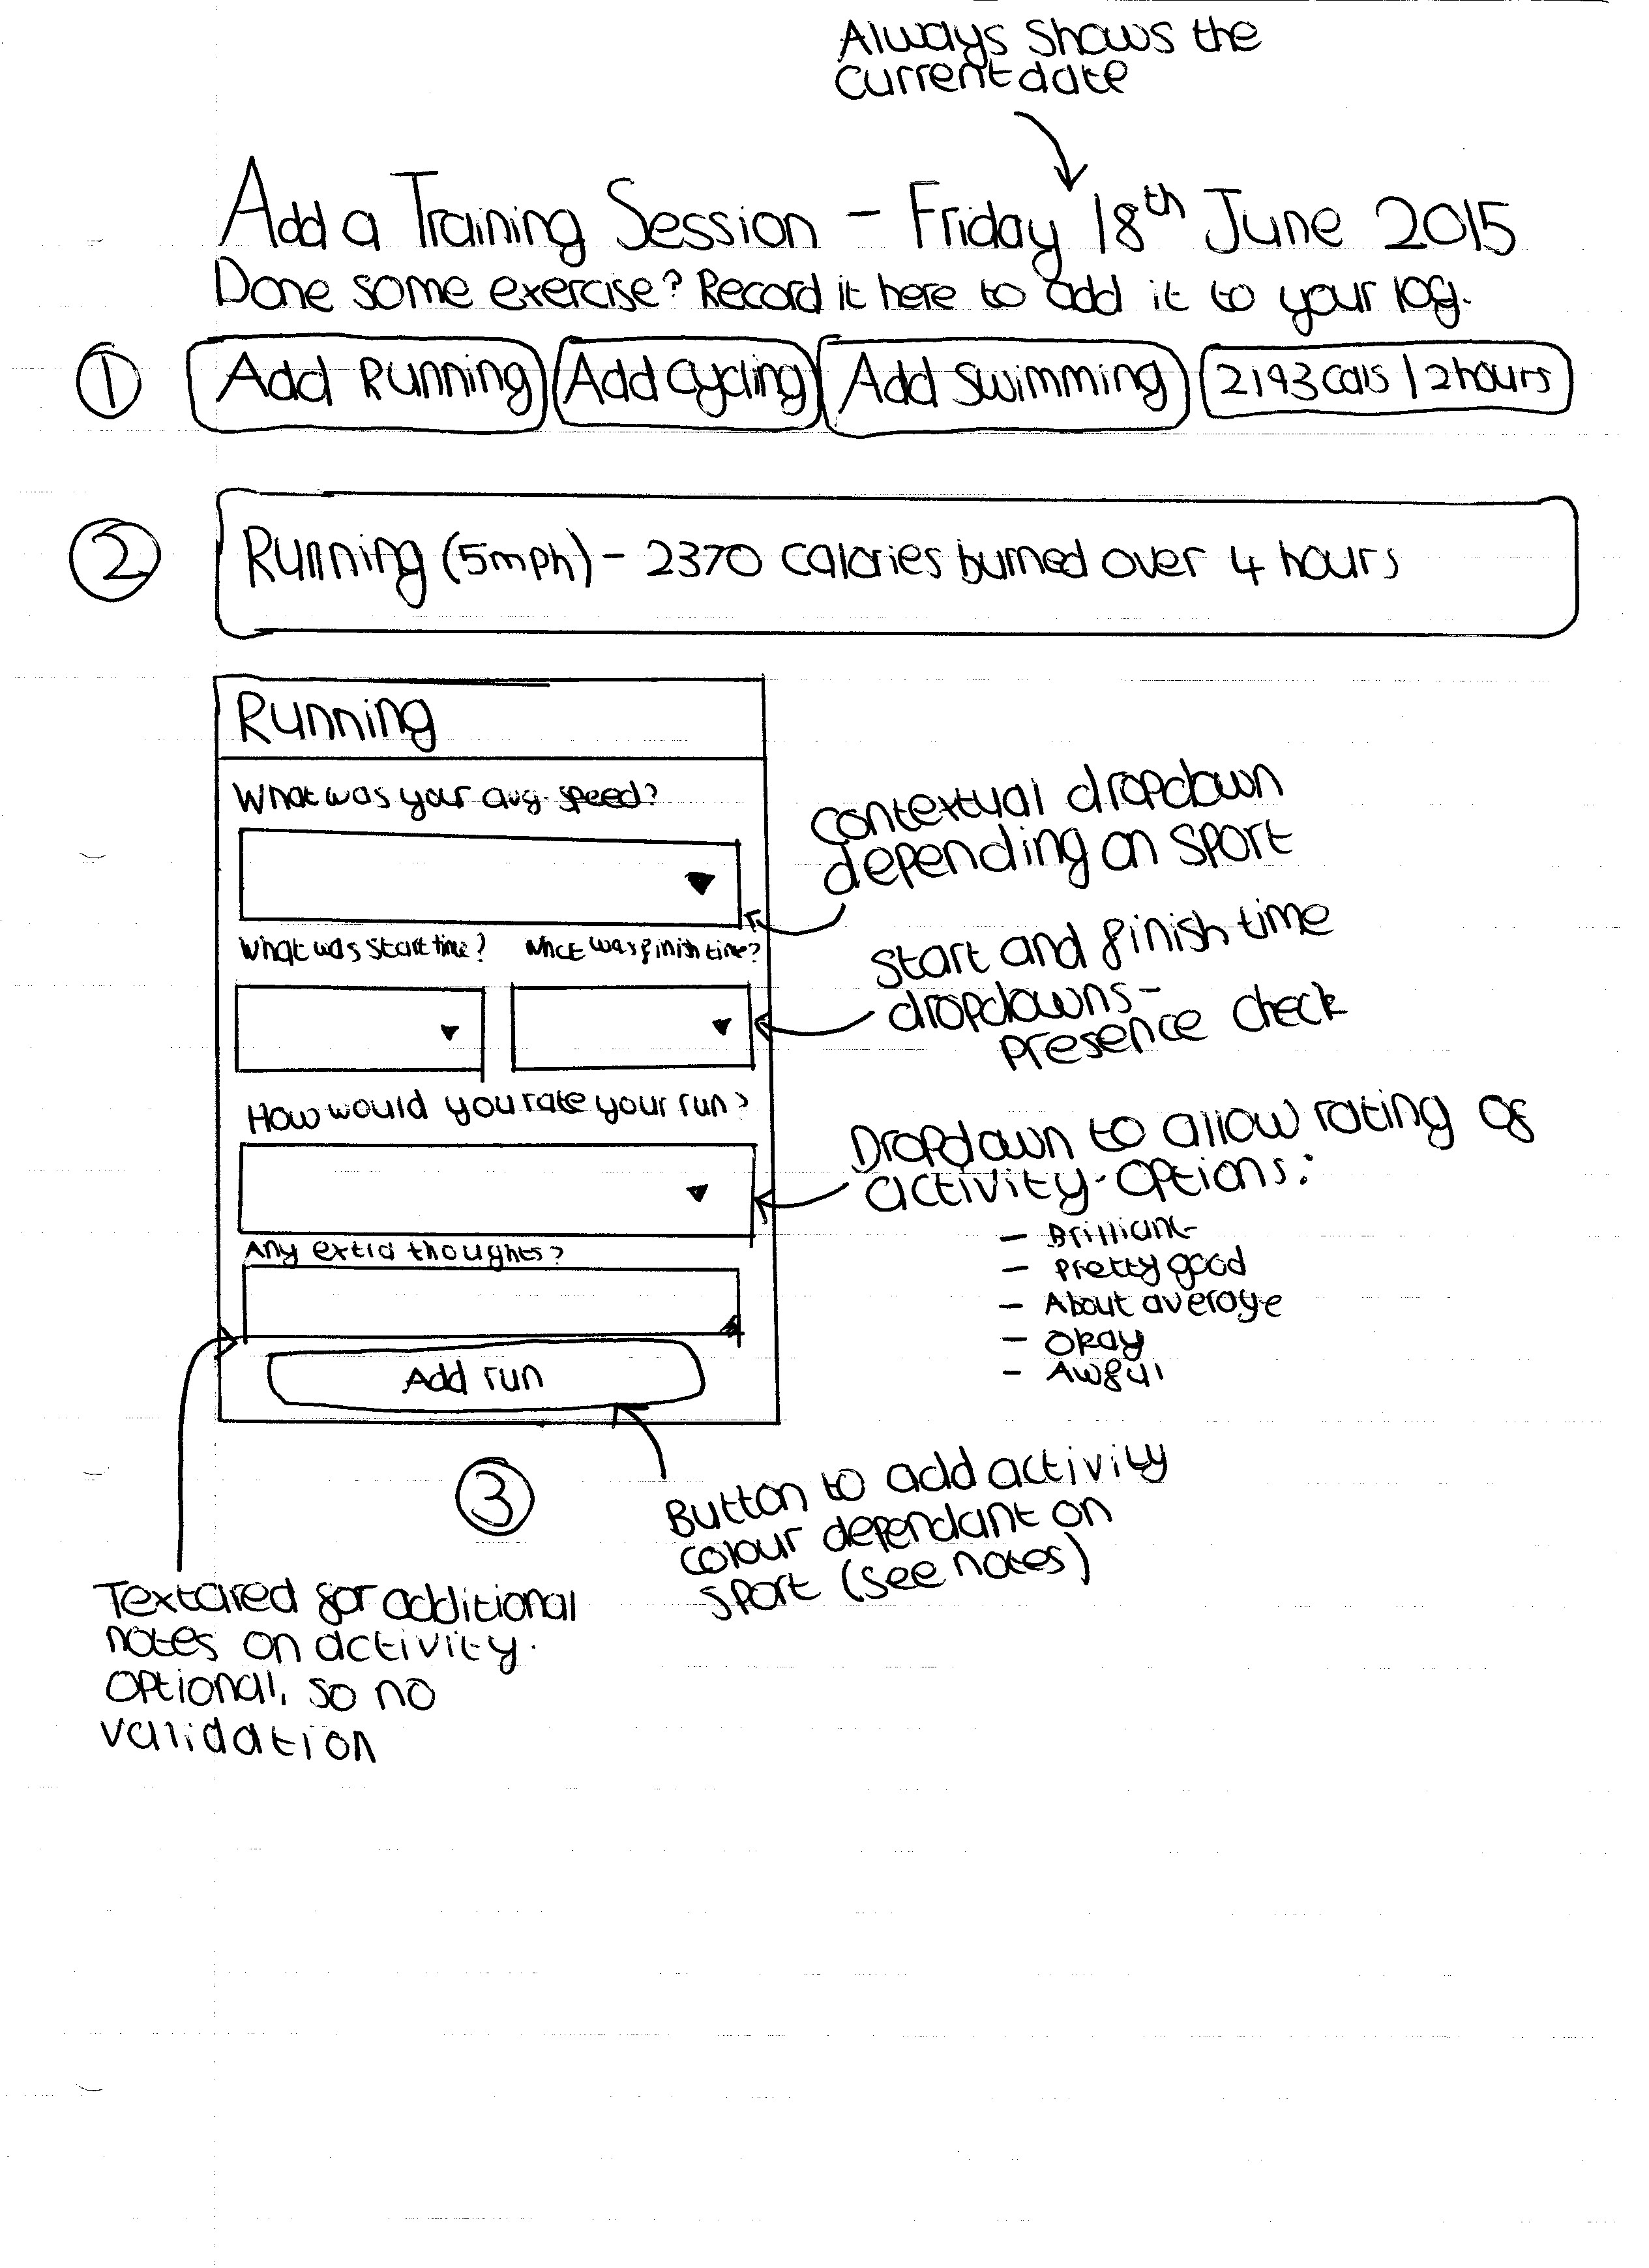
\includegraphics[scale=0.55]{design_ui/add_training}
\end{figure}
\clearpage

\subsection{Profile Page}
\begin{figure}[h!]
  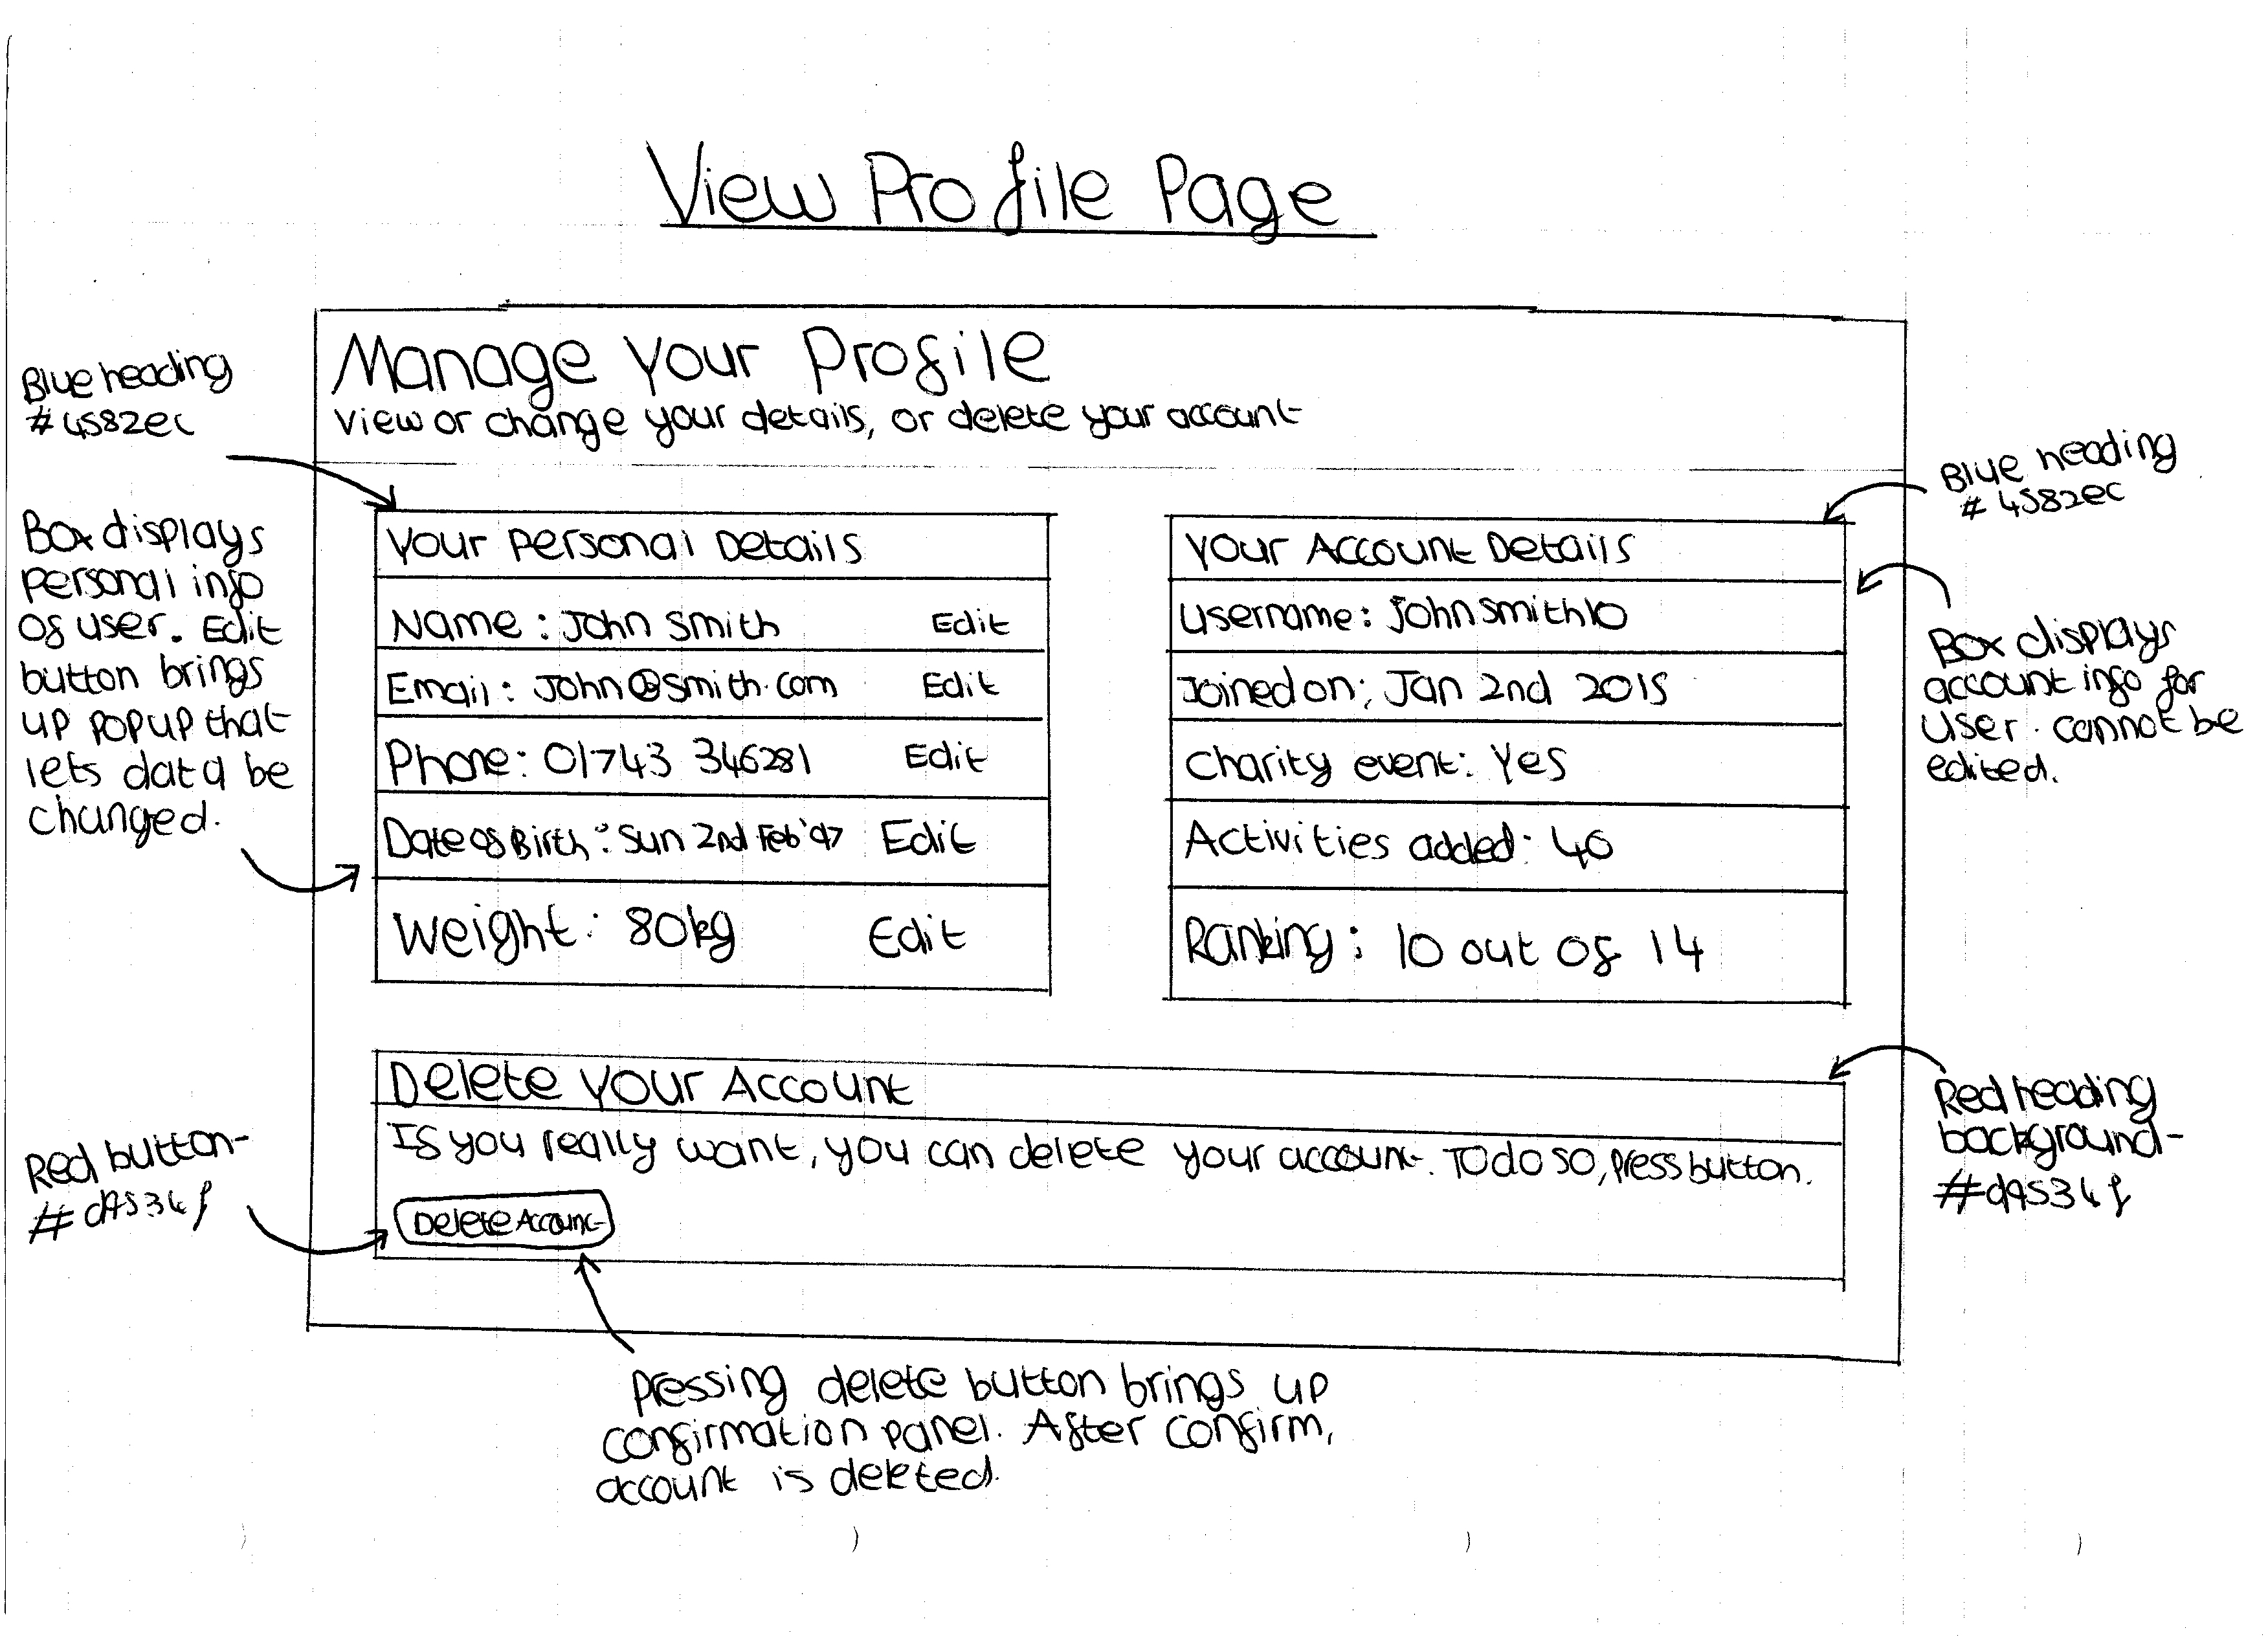
\includegraphics[scale=0.55]{design_ui/profile}
\end{figure}
\clearpage

\subsection{Charity Team Ranking Page}
\begin{figure}[h!]
  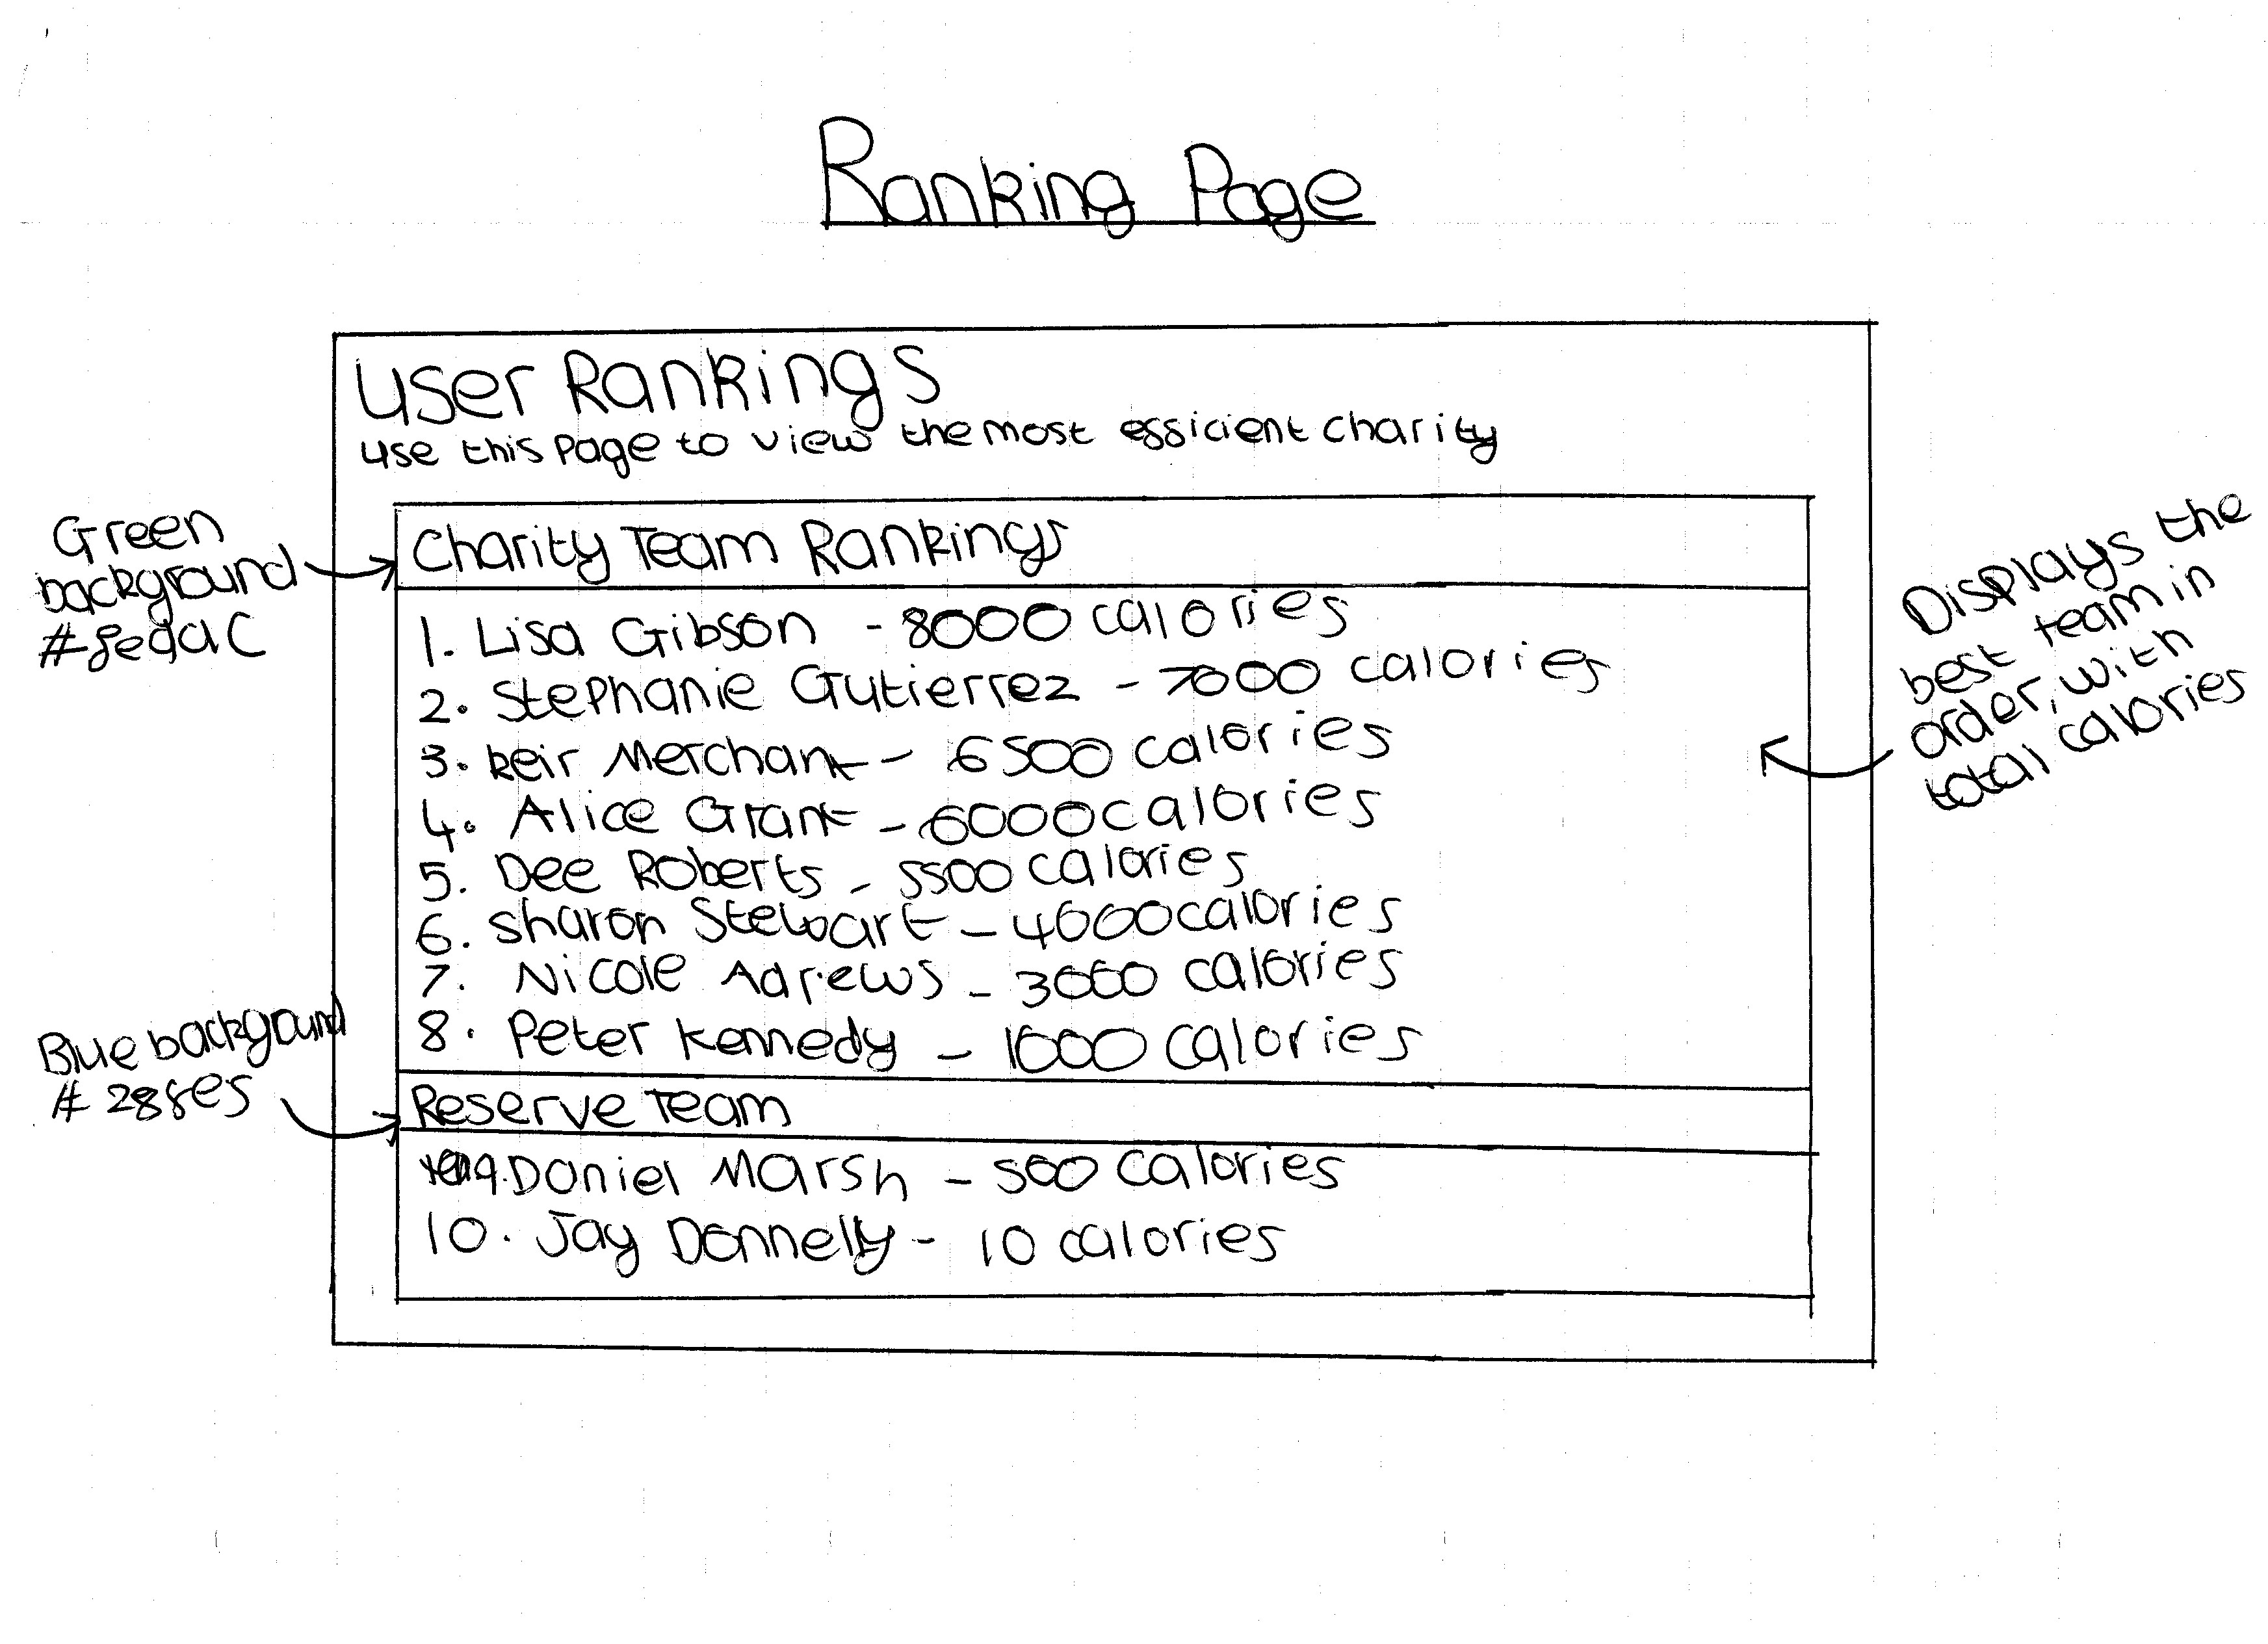
\includegraphics[scale=0.55]{design_ui/rankings}
\end{figure}
\clearpage

\subsection{Page Linkages}
The following diagram shows how the different pages of the system link together.


\section{Hardware and Software Requirements}
In order for the system to function correctly, a minimum level of hardware, and some certain software, is needed.

\subsection{Hardware}
The system is a web application, and as such requires a stable internet connection to function correctly; therefore, the device used to access the system will need support for the internet, either through a wireless card or an ethernet connection. As a web application, the system can be used on both traditional computing devices, such as desktop PCs and laptops, as well as smart phones and tablets. If using a non touch device, the system has been designed for screens at least 17" in size - a resolution of 1280x1024. The system will function at smaller displays than this, but has not been fully tested as such. Desktops will also requires a mouse, in order to point at and click elements on the page; any mouse is suitable for this task. Additionally, a keyboard is needed for data entry. Laptops usually come with trackpads and keyboards built in, so the need for these additional peripherals is reduced.

If the user is using a smart phone or tablet - a scenario that is likely, as the audience is a group not known for sitting down at a desk all day - no additional hardware is needed, as the device would come with everything built in, such as a touch screen for interacting with element and a virtual keyboard for data entry. The same internet connection requirements apply.

\subsection{Software}
As a web application, a web browser is the only piece of software needed to access the system - the user need simply visit the correct web address, and they can access the system. The most suitable browser to open the system in is Google Chrome; luckily, this also happens to be the most popular browser worldwide, so it is likely that they runners are already using it.

 Chrome boasts superior rendering technology to other browsers, as well as greater performance; in addition, all the testing of the system has been performed in Chrome, so it is possible that the system may not function correctly if used in other browsers. 

 Additionally, the user will need an operating system installed on their computer. Google Chrome is available for Windows, OSX and all Debian/Red Hat distributions of Linux, so their choice of operating system does not matter.

\section{Processing Stages}
This section documents the large range of processes that go into making the system function correctly. It has been split up into a number of sections for organisation. For Python/web development constructs in general that the examiners may find themselves unfamiliar with, an explanation in English has been provided.

\subsection{Global Processes}
A number of processes have been used multiple times throughout the system, such as routing and validation. To avoid writing them out every time they occur, they have been documented here.

\subsubsection{Routing}
The concept of \textit{routing} is fundamental to a Flask application. Practically every function is linked to a route, and every route is linked to a URL. For example, the function auth.login is linked to the URL ``/login'', as makes logical sense. Therefore, visiting the URL ``/login'' will run the code in the function auth.login. 

\begin{verbatim}
@file.route('/url', methods=[METHODS])
begin function route_name:
  begin route logic
  return route result
\end{verbatim}
As can be seen, each route is made up of a number of elements. \textit{file} is equivalent to the file in which the route appears; for example, the function auth.login is in auth.py, therefore its \textit{file} parameter would be set to \textit{auth}. The \textit{url} paramater is equivalent to the URL that the route links to, so for auth.login it would be ``/login'', as written above.

The \textit{methods} parameter specifies which HTTP method(s) can be used to access the route - either \textit{GET}, \textit{POST}, or a combination of the two. A detailed discussion on the differences between the the two is beyond the scope of this explanation, but, put simply, a route with only \textit{GET} specified is designed to be accessed by the user, whereas those with \textit{POST} are designed for the server (in this system, they are always AJAX routes). A route with both \textit{GET} and \textit{POST} is designed to be accessed by the user, but it also sends data to the server.

The route logic is the main code for the route. In auth.login, for example, it contains processing to check that their are no validation errors on the form, and for logging the user in. Every route returns something. For routes with just \textit{GET} or both \textit{GET} and \textit{POST}, this will always be a Jinja2 HTML template, which is then rendered by the browser. For purely \textit{POST} routes, often a JSON object or dictionary is returned, but this varies; see the individual route processes for details.

\subsection{AJAX Calls}
AJAX, which stands for \textit{Asynchronous JavaScript and XML}, is a method by which the rendered HTML can interact with the Python server without having to reload the page, creating a smooth experience. The syntax is as follows:

\begin{verbatim}
$.ajax({
  url: `/ajax/ROUTE',
  type: `POST',
  dataType: `DATA_TYPE',
  contentType: `CONTENT_TYPE'
  data: `DATA',
  success: function (data) {
    CALLBACK(data);
  }
});
\end{verbatim}

\section{Evaluation Criteria}

\cleardoublepage


\part{Program Documentation}

\section{User Interface}
This section contains screen captures of all different areas of the completed the system, along with additional notes stating how they are fit for purpose.

\subsection{Main Layout}
Every other page derives constant elements, like the navigation bar and footer, from this template, to ensure visual consistency.

\begin{figure}[h!]
  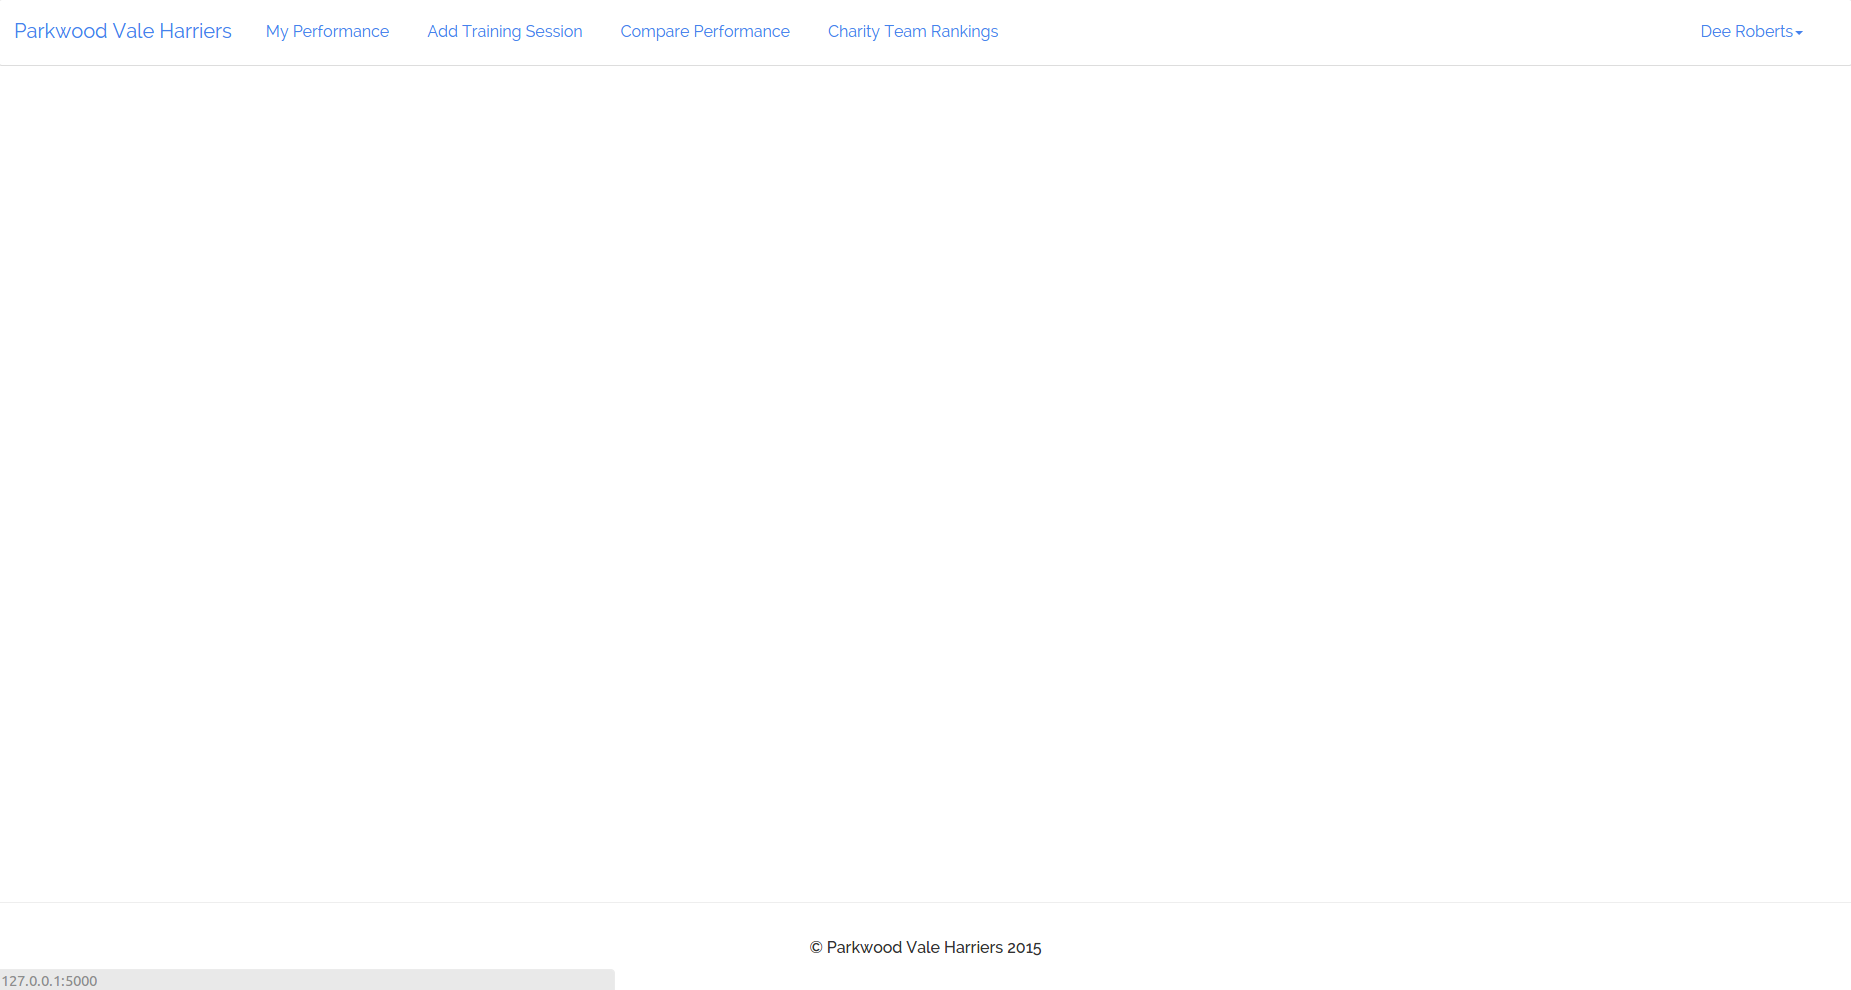
\includegraphics[scale=0.30]{final_ui/layout}
  \caption{Master Layout}
\end{figure}

\subsection{Register Page}
The register page features a clear, simple design, with input boxes laid out in a consistent style. Each input box features placeholder text, to provide a visual guide to user as to what sort of data they should be typing in. To simplify entry, date of birth input brings up a datepicker widget upon click, making it simple for users to enter their date of birth. Additionally, validation errors are featured at top of page in a big yellow box, making them easy to see; they also have a close button to prevent them getting in way. A link to login page allows users who already have an account to quickly login.

\begin{figure}[h!]
  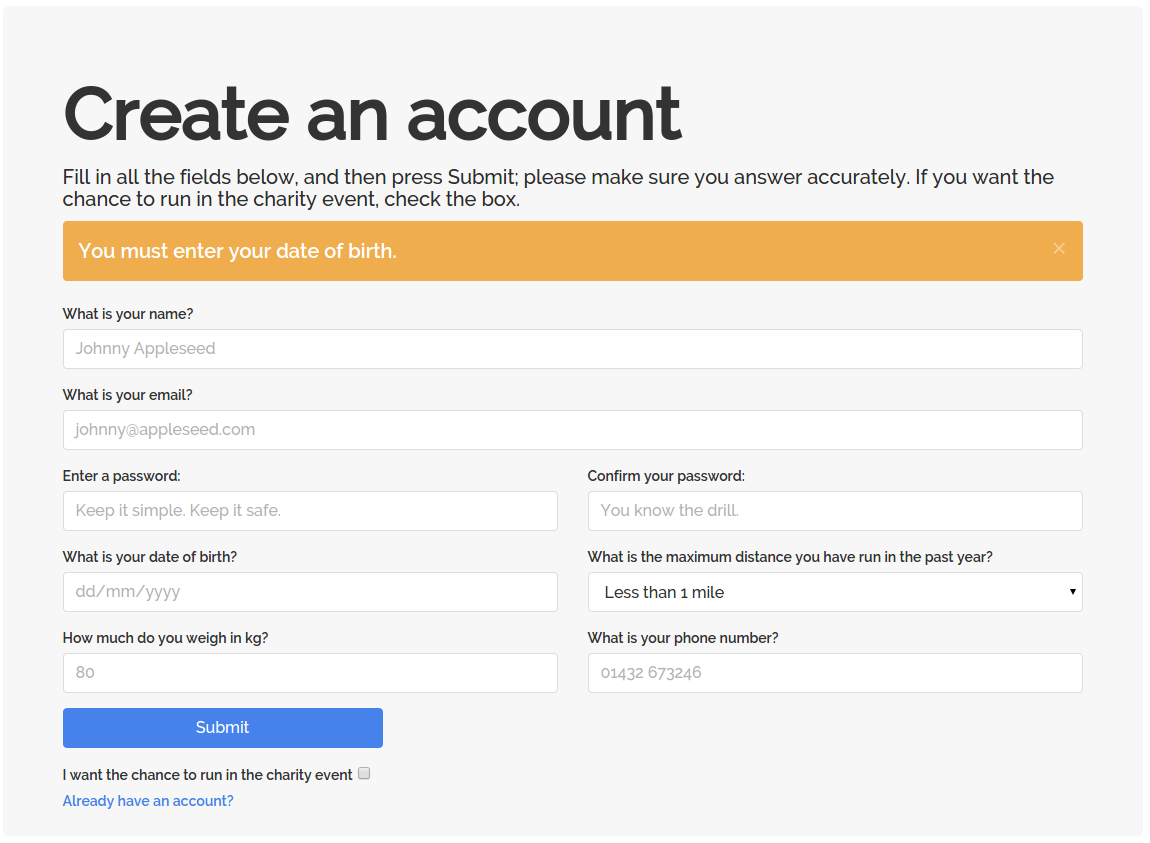
\includegraphics[scale=0.35]{final_ui/register}
  \caption{Registration Page}
\end{figure}
\clearpage

\subsection{Login Page}
As login page has only one function - to get user logged in to system - it features a very simple layout, with only two input forms and a button. Like registration form, though not visible in this capture, placeholders are overlaid on inputs to provide a visual guide as to should be typed in. Additionally, password field blanks out input, a helpful security measure that prevents onlookers viewing user's password. For consistency, same validation error system as with registration page is used.

\begin{figure}[h!]
  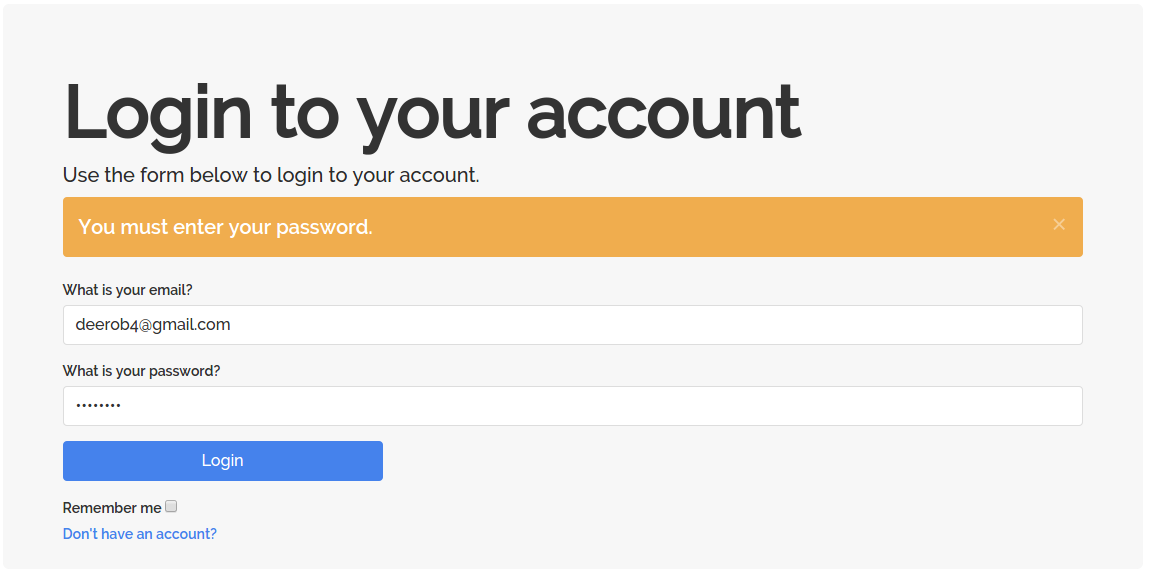
\includegraphics[scale=0.35]{final_ui/login}
  \caption{Login Page}
\end{figure}
\clearpage

\subsection{Profile Page}
profile page allows user to view and update their personal information. Certain sections appear on demand, so multiple captures have been taken.

\subsubsection{Main View}
Due to large amount of data that is being presented on this page, a structured approach has been taken, with a three-panel view being implemented. This helps to seperate different areas of page in a logical manner, making it easier for user to find what they are looking for. Each item of data is given its own row, making it clear which is which. delete account section has been coloured in red, a colour traditionally associated with danger. This helps to convey to user that bad things will happen if they delete their account. Furthermore, playful text has been used in delete account panel, to bring a sense of amusement and, hopefully, dissuade user from following through with their actions.

\begin{figure}[h!]
  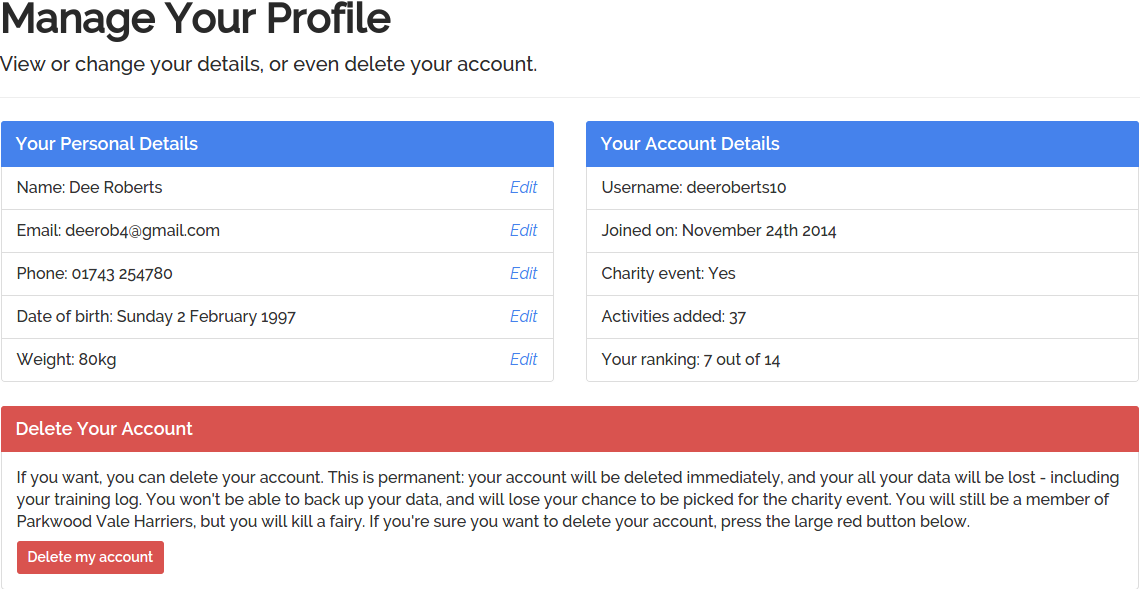
\includegraphics[scale=0.35]{final_ui/profile}
  \caption{Profile Page - Main View}
\end{figure}
\clearpage

\subsubsection{Change Details}
interface for changing details is very simple - it features just an input for changing element, and a button to confirm. placeholder text for input is set to current item, for visual consistency. Making this panel pop up as opposed to being on a seperate page improves flow of page, preventing user becoming disorientated.

\begin{figure}[h!]
  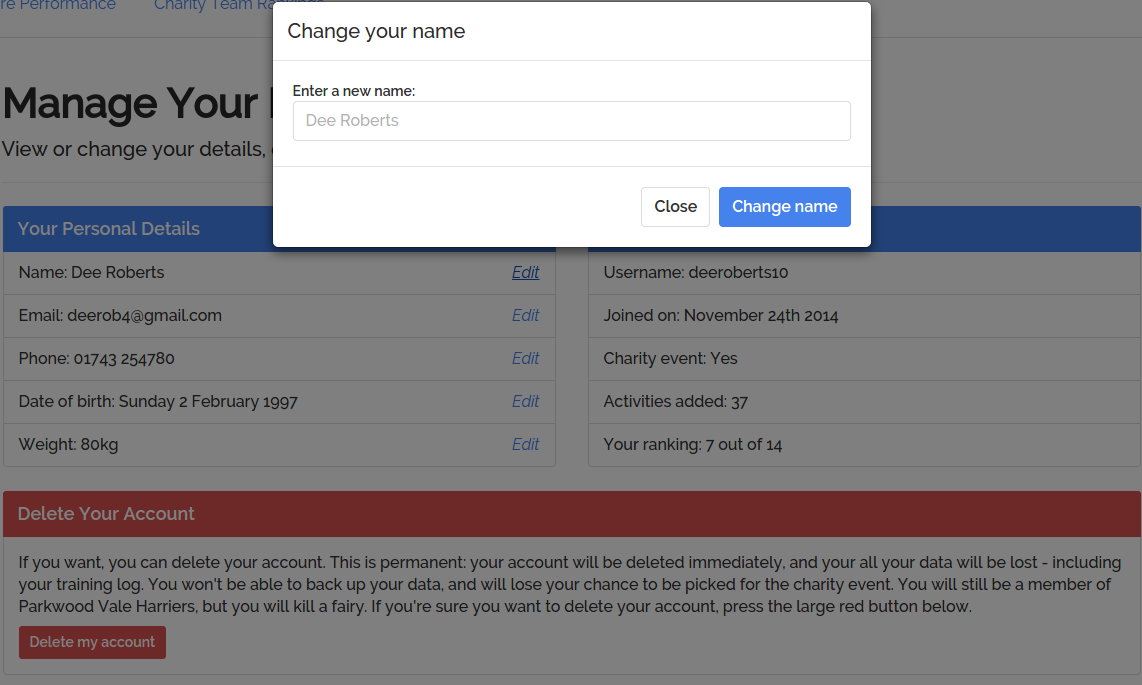
\includegraphics[scale=0.35]{final_ui/profile_change}
  \caption{Profile Page - Change Details}
\end{figure}
\clearpage

\subsubsection{Delete Account}
To ensure that user is fully aware of severity of deleting their account, they must type in ``I will lose everything'' into box; this also makes it harder for them to accidentally delete their account. Positive reinforcement is used in this section through use of colours - greeen is associated with positivity, and users have been shown to click on green coloured buttons more often than red; this further dissuades them from deleting their account.

\begin{figure}[h!]
  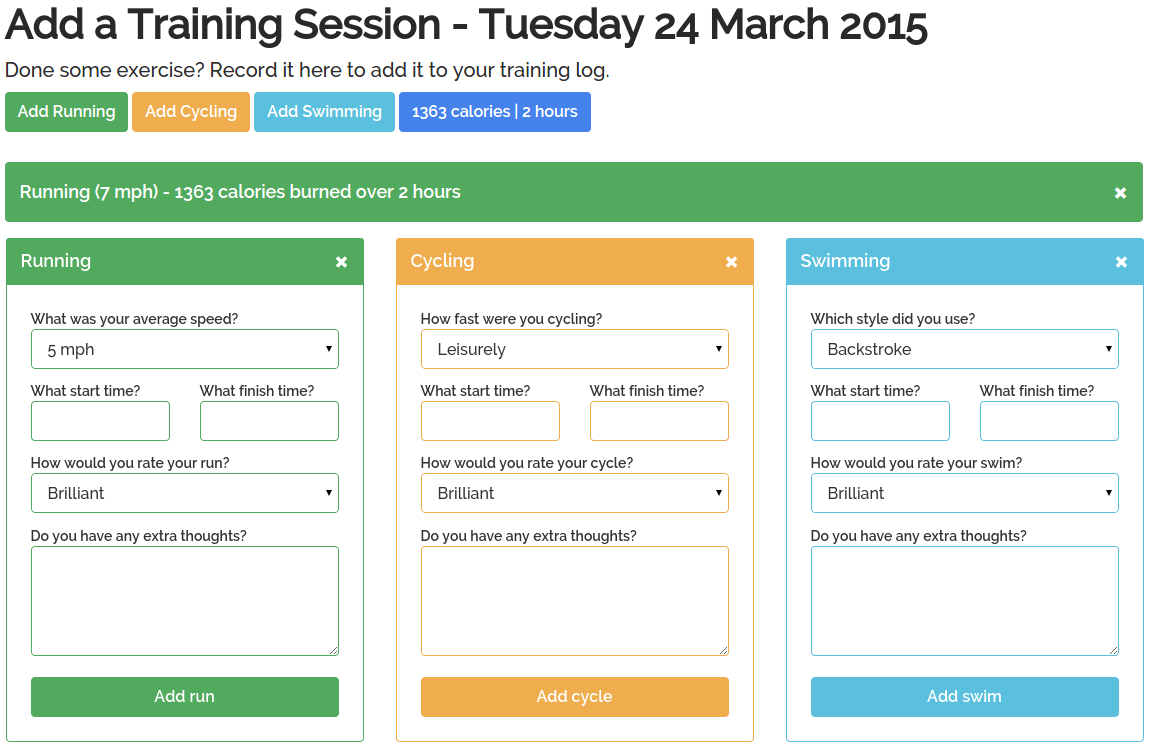
\includegraphics[scale=0.35]{final_ui/account_delete}
  \caption{Profile Page - Delete Account}
\end{figure}
\clearpage

\subsection{User Performance Page}
The user performance page is the main page of the system, and is the first page the user sees when they log into the system.

\begin{figure}[h!]
  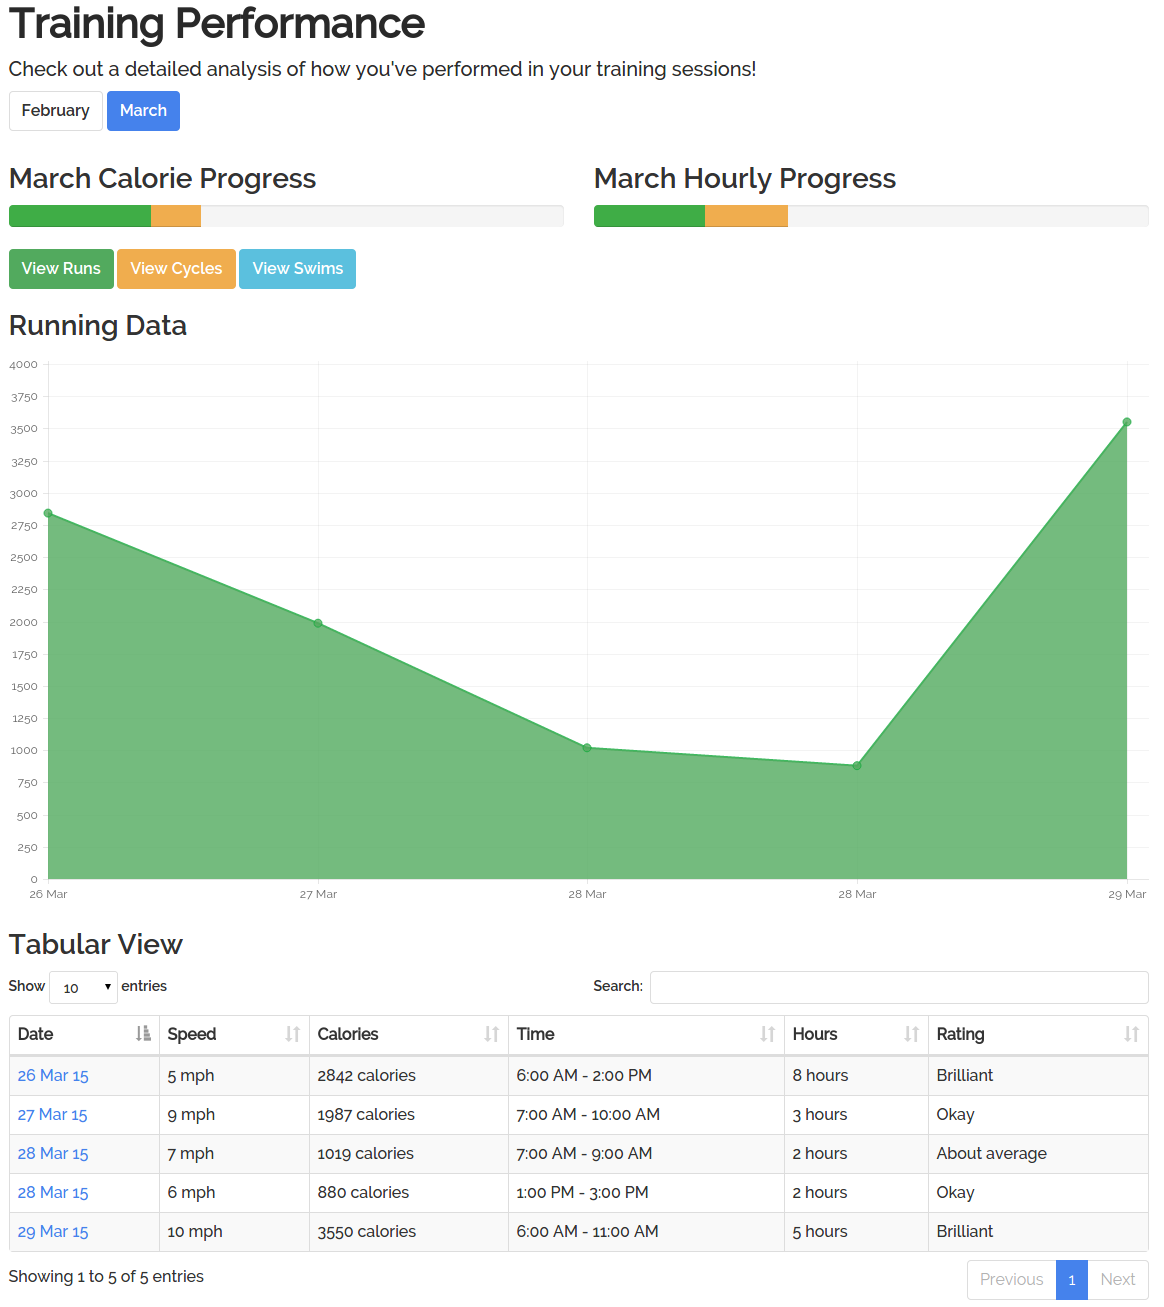
\includegraphics[scale=0.35]{final_ui/user_performance}
  \caption{User Performance Page}
\end{figure}
\clearpage

To prevent the user being overloaded with data, the performance data is seperated into months, with a different URL for each month - ``/performance/march'' to view performance for March, for example. By default, the user is automatically taken to the page for the current month, ensuring that they always see the most up to date data. Buttons are available at the top to switch between months; notably, only months where training sessions have been added are visible, ensuring that the user never sees blank data - something which could be discouraging to the runner.

It allows the user to view a number of elements relating to their performance in the three sports. The two bars at the top display a simple view of how far the user is to reaching their goal for the month. The different sports that make up goal progress are shown through colours - green for running, yellow for cycling and blue for swimming, as in the rest of the application. Not shown in the capture are the popups that appear when the user hovers over the bars - these display the number of calories / hours that make up the bars. 

All of the sessions the user has done in each sport is plotted on a line chart, allowing for easy visualisation of trends over the month; this makes it very easy for the user to see how they are doing, a feature that runners would find very helpful When each plot point is moused over, the exact number of calories are shown. There are three different graphs for each sport; these are changed by clicking the colour coded buttons at the top of the graph. When switching sport, the entire section smoothly slides out, allowing the new one to slide in. By providing such a seamless animation, the user is provided with a sense of place within the system, improving its ease of use.

The page also shows each training session the user has performed in the selected sport in a table. The table shows all the information about the training session, allowing the user gain a detailed understanding of how they are progressing - something that is important when training for a charity event. The tables allow for the number of entries shown to be limited, introducing an element of pagination. This allows the user to control how many sessions they see at once, keeping them orientated within the view. The tables can also be sorted by clicking on the headers, allowing the user greater control over how they view the sessions; they are listed in date order by default, as the user would expect.

Additionally, and perhaps most helpfully, the tables allow for the user to search for specific training sessions. This would be particularly helpful if a user wished to find all sessions that they rated as brilliant, or all on a particulary day - they would just have to type the term into the search box, and the data is automatically filtered.

\clearpage

\subsection{Add Activity Page}

\begin{figure}[h!]
  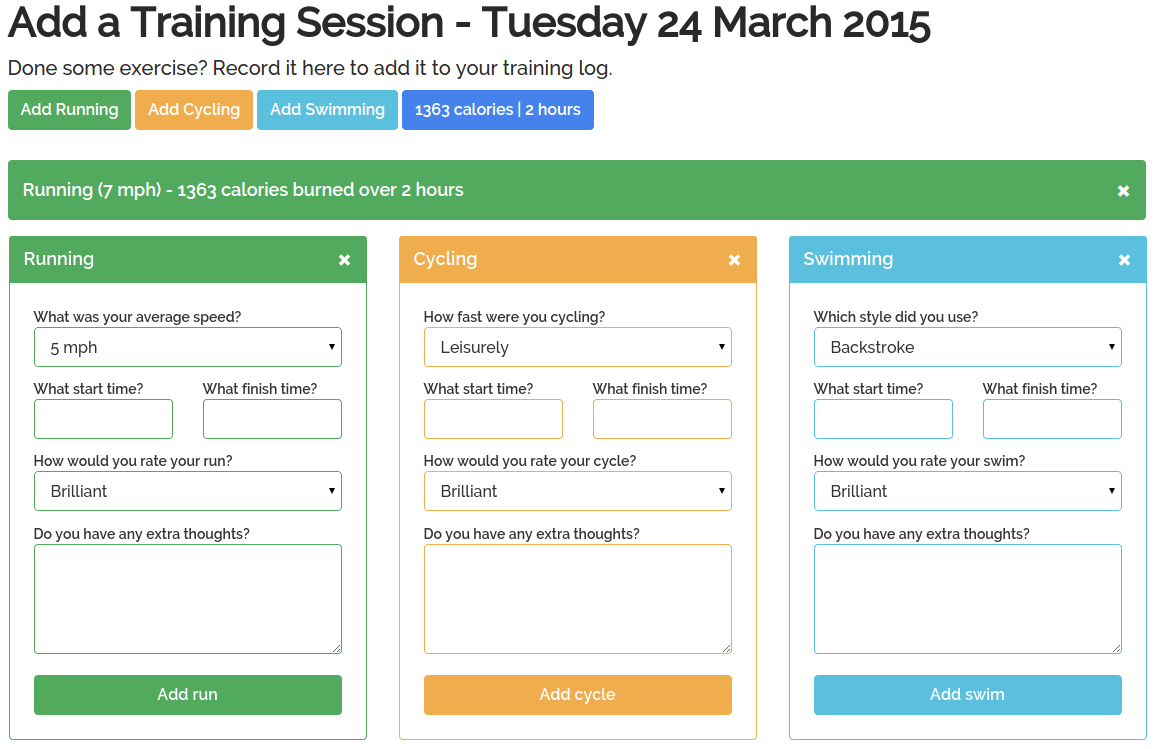
\includegraphics[scale=0.35]{final_ui/add_activity}
  \caption{Add Activity Page}
\end{figure}

\clearpage

\subsection{Rankings Page}

\begin{figure}[h!]
  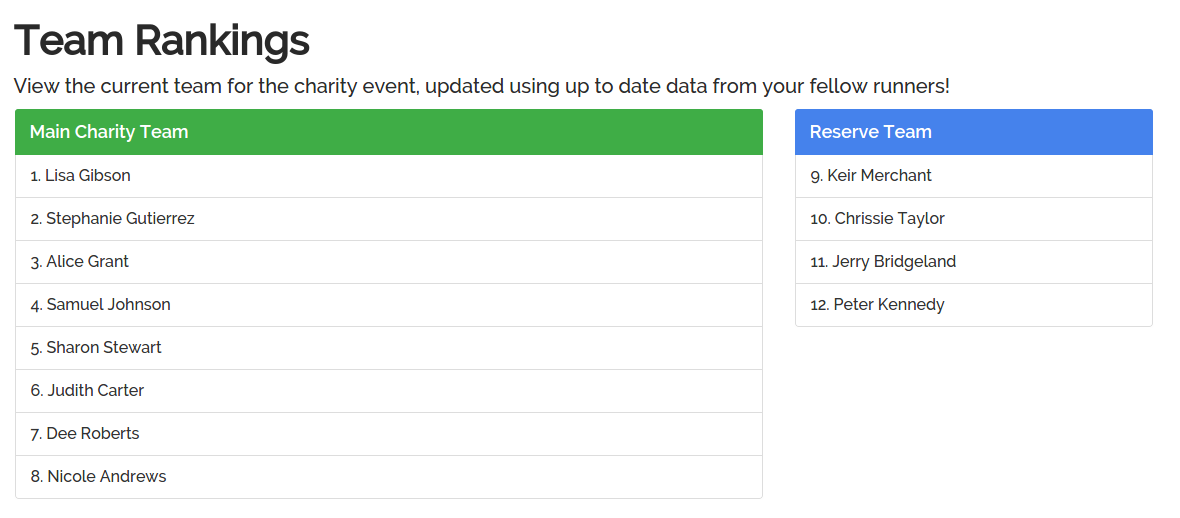
\includegraphics[scale=0.35]{final_ui/rankings}
  \caption{Rankings Page}
\end{figure}

\section{Database Models}
This section contains documentation on finished database tables and models, including an ER diagram showing relationship between tables, schematics, and a visual view.

\subsection{Table Relationships}
The activities and users are linked through a foreign key. This means that there is a one to many relationship between users and activities - one user can have many activities, but each activity can only have one user.

\begin{figure}[h!]
  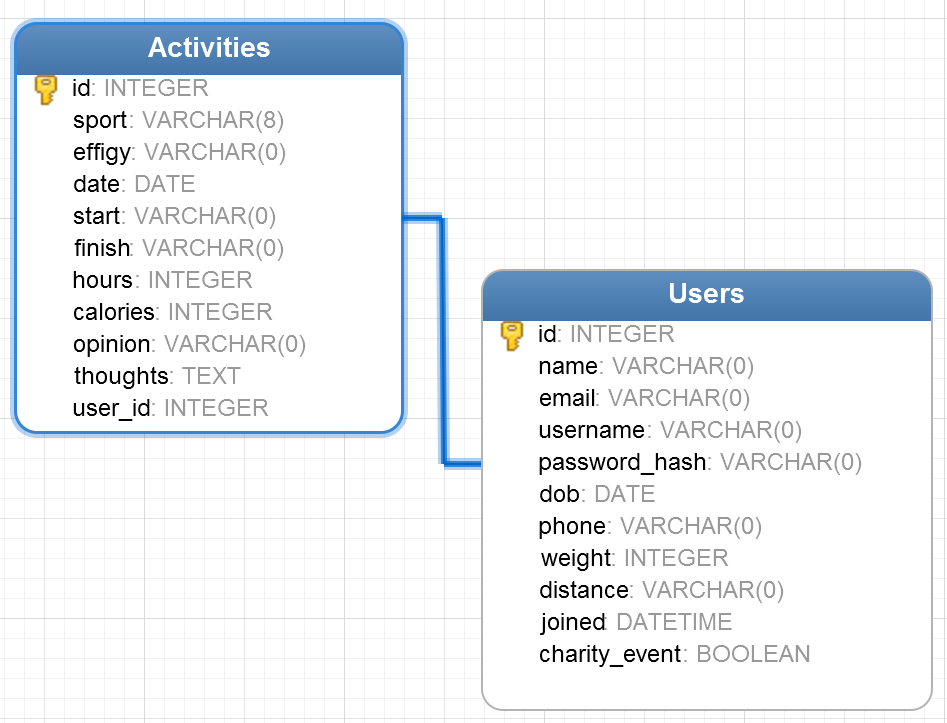
\includegraphics[scale=0.5]{images/database/er_diagram}
  \caption{Table Relationships}
\end{figure}

\clearpage

\subsection{Table Schemas}
Each table in database has its own schema, in which is described name, data type and key type of each column. They can be found below.

\subsubsection{Users Table}
id column is primary key. Email is used to login. Username is used in certain routes; see processes. Weight is used to calculate calories.
\begin{figure}[h!]
  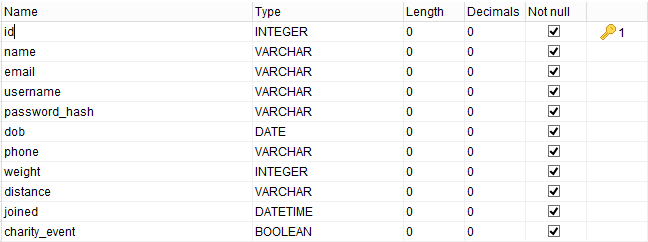
\includegraphics[scale=0.65]{images/database/users_schema}
  \caption{Users Table Schema}
\end{figure}

\subsubsection{Activities Table}
id column is primary key. Effigy is specific details of each activity, such as swimming stroke or running speed. user\_id is foreign key linking activity to a user.
\begin{figure}[h!]
  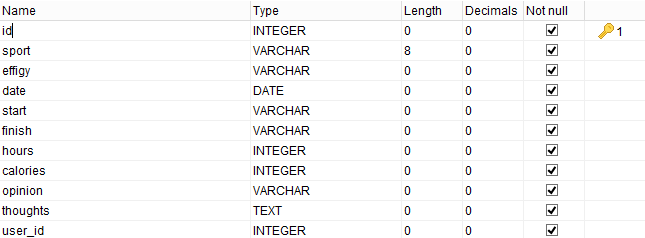
\includegraphics[scale=0.65]{images/database/activities_schema}
  \caption{Activities Table Schema}
\end{figure}

\clearpage

\subsection{Data Views}
following is a snapshot of data in two tables at time of writing, to illustrate how they will appear in production.

\subsubsection{Users Table}
\begin{figure}[h!]
  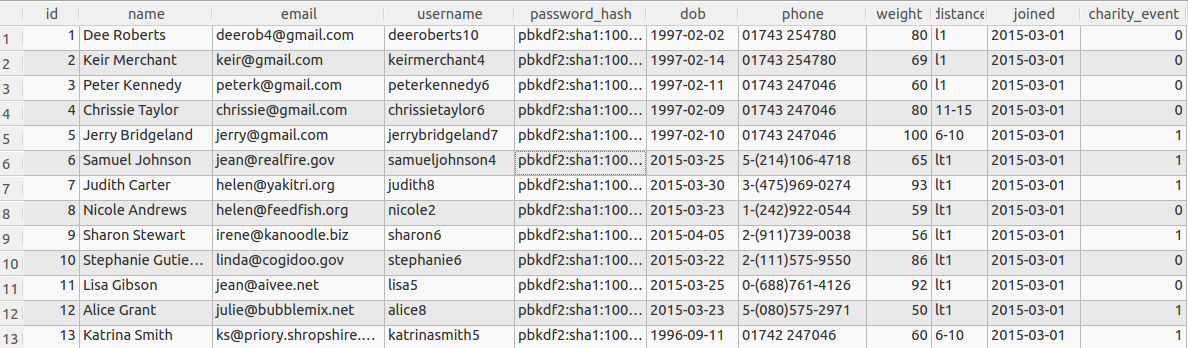
\includegraphics[scale=0.37]{images/database/users_visual}
  \caption{Users Table Data View}
\end{figure}

\subsubsection{Activities Table}
\begin{figure}[h!]
  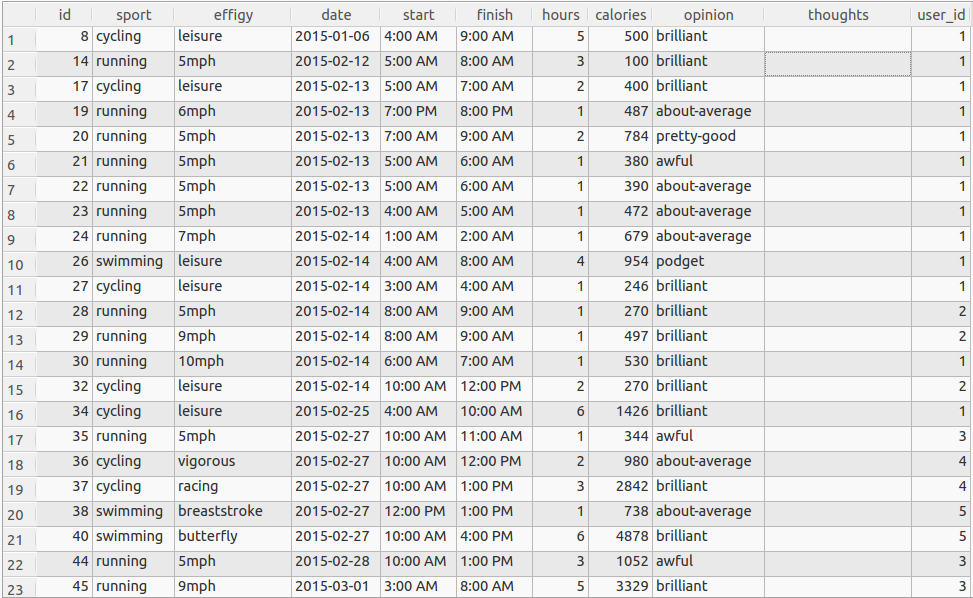
\includegraphics[scale=0.37]{images/database/activities_visual}
  \caption{Activities Table Data View}
\end{figure}

\section{Variables}
A very large number of variables have been used throughout system in order to store data temporarily. It should be noted that variables in Python do not work in same way as in other languages like Visual Basic: a variable acts as a pointer to something already in memory (created by Python automatically), as opposed to creating a space in memory to store contents of variable. Therefore, the code x = 10 merely sets variable x to an address that points at 10, as opposed to writing 10 into memory.

\subsection{Global Variables}
Throughout system, a small number of global variables are used in order to provide functionality. following table lists their names, type and purpose.
\begin{table}[h]
\begin{tabular}{|l|l|l|}
\hline
\textbf{Name} & \textbf{Type} & \textbf{Purpose}                        \\ \hline
login\_manager                    & Object                 & Creates actual Flask application object.     \\ \hline
db                     & Object                 & Returns a connection to database.            \\ \hline
User                   & Object                 & Creates a connection to Users db table.      \\ \hline
Activity               & Object                 & Creates a connection to Activities db table. \\ \hline
current\_user          & Object                 & Returns details about logged in user.        \\ \hline
\end{tabular}
\caption{Global Variables}
\end{table}

\subsection{Local Variables}
The following table contains a list of all variables used locally throughout the system's functions and classes.
\begin{longtable}{|l|l|l|l|l|}
\hline
\textbf{Name}   & \textbf{Type} & \textbf{File Found} & \textbf{Function}       & \textbf{Purpose}                \\ \hline
name            & Object        & forms.py            & MemberForm              & Creates name input.         \\ \hline
dob             & Object        & forms.py            & MemberForm              & Creates dob input.          \\ \hline
password        & Object        & forms.py            & MemberForm              & Creates password input.     \\ \hline
confirm         & Object        & forms.py            & MemberForm              & Creates confirm input.      \\ \hline
charity\_event  & Object        & forms.py            & MemberForm              & Creates charity input.      \\ \hline
distance        & Object        & forms.py            & MemberForm              & Creates distance input.     \\ \hline
weight          & Object        & forms.py            & MemberForm              & Creates weight input.       \\ \hline
phone           & Object        & forms.py            & MemberForm              & Creates phone input,        \\ \hline
submit          & Object        & forms.py            & MemberForm              & Creates submit button.      \\ \hline
age             & int           & forms.py            & validate\_dob           & Stores user's age.          \\ \hline
email           & Object        & forms.py            & LoginForm               & Creates email input.        \\ \hline
password        & Object        & forms.py            & LoginForm               & Creates password input.     \\ \hline
remember        & Bool          & forms.py            & LoginForm               & Creates remember input.     \\ \hline
login           & Object        & forms.py            & LoginForm               & Creates login button.       \\ \hline
id              & Object        & models.py           & User                    & Creates id column.          \\ \hline
name            & Object        & models.py           & User                    & Creates name column.        \\ \hline
email           & Object        & models.py           & User                    & Creates email column.       \\ \hline
username        & Object        & models.py           & User                    & Creates username column.    \\ \hline
password\_hash  & Object        & models.py           & User                    & Creates hash column.        \\ \hline
dob             & Object        & models.py           & User                    & Creates dob column.         \\ \hline
phone           & Object        & models.py           & User                    & Creates phone column.       \\ \hline
weight          & Object        & models.py           & User                    & Creates weight column.      \\ \hline
distance        & Object        & models.py           & User                    & Creates distance column.    \\ \hline
joined          & Object        & models.py           & User                    & Creates joined column.      \\ \hline
charity\_event  & Object        & models.py           & User                    & Creates charity column.     \\ \hline
activities      & Object        & models.py           & User                    & Creates relationship property.  \\ \hline
id              & Object        & models.py           & Activity                & Creates id column.          \\ \hline
sport           & Object        & models.py           & Activity                & Creates effigy column.      \\ \hline
date            & Object        & models.py           & Activity                & Creates date column.        \\ \hline
start           & Object        & models.py           & Activity                & Creates start column.       \\ \hline
finish          & Object        & models.py           & Activity                & Creates finish column.      \\ \hline
hours           & Object        & models.py           & Activity                & Creates hours column.       \\ \hline
calories        & Object        & models.py           & Activity                & Creates calories column.    \\ \hline
opinion         & Object        & models.py           & Activity                & Creates opinion column.     \\ \hline
thoughts        & Object        & models.py           & Activity                & Creates thoughts column.    \\ \hline
user\_id        & Object        & models.py           & Activity                & Creates user\_id column.    \\ \hline
today           & Date          & helpers.py          & calculate\_age          & Stores current date.        \\ \hline
months          & List          & perf\_data.py       & perf\_data              & Stores a list of months.        \\ \hline
all\_runs       & Object        & per\_data.py        & perf\_data              & Stores all user's runs.     \\ \hline
all\_cycles     & Object        & per\_data.py        & perf\_data              & Stores all user's cycles.   \\ \hline
all\_swims      & Object        & per\_data.py        & perf\_data              & Stores all user's swims.    \\ \hline
month\_map      & Dict          & per\_data.py        & perf\_data              & Maps months to integers.        \\ \hline
calorie\_goal   & int           & per\_data.py        & perf\_data              & Stores calorie goal.        \\ \hline
hour\_goal      & int           & per\_data.py        & perf\_data              & Stores hourly goal.         \\ \hline
sport             & String      & ajax.py        & sport\_block        & Stores type of sport                \\ \hline
sport             & String      & ajax.py        & send\_activity      & Retrieves sport                     \\ \hline
effiy             & String      & ajax.py        & send\_activity      & Retrieves effigy                    \\ \hline
hours             & int         & ajax.py        & send\_activity      & Retrieves hours                     \\ \hline
start             & int         & ajax.py        & send\_activity      & Retrieves start                     \\ \hline
finish            & int         & ajax.py        & send\_activity      & Retrieves finish                    \\ \hline
opinion           & String      & ajax.py        & send\_activity      & Retrieves opinion                   \\ \hline
thoughts          & String      & ajax.py        & send\_activity      & Retrieves thoughts                  \\ \hline
activity          & Object      & ajax.py        & send\_activity      & Stores completed activity           \\ \hline
activity\_id      & int         & ajax.py        & remove\_activity    & Stores id of activity           \\ \hline
base\_calories    & Dict        & ajax.py        & calculate\_calories & Stores base calorie values          \\ \hline
sport             & String      & ajax.py        & calculate\_calories & Retrieves sport                     \\ \hline
effiy             & String      & ajax.py        & calculate\_calories & Retrieves effigy                    \\ \hline
hours             & int         & ajax.py        & calculate\_calories & Retrieves hours                     \\ \hline
start             & int         & ajax.py        & calculate\_calories & Retrieves start                     \\ \hline
finish            & int         & ajax.py        & calculate\_calories & Retrieves finish                    \\ \hline
opinion           & String      & ajax.py        & calculate\_calories & Retrieves opinion                   \\ \hline
thoughts          & String      & ajax.py        & calculate\_calories & Retrieves thoughts                  \\ \hline
base\_value       & int         & ajax.py        & calculate\_calories & Stores activity base value      \\ \hline
calories          & int         & ajax.py        & calculate\_calories & Stores total calories               \\ \hline
modifier          & int         & ajax.py        & calculate\_calories & Stores calorie modifier     \\ \hline
activity\_data    & Dict        & ajax.py        & calculate\_calories & Stores all activity data            \\ \hline
sport             & String      & ajax.py        & sport\_block        & Stores type of sport                \\ \hline
sport             & String      & ajax.py        & send\_activity      & Retrieves sport                     \\ \hline
effiy             & String      & ajax.py        & send\_activity      & Retrieves effigy                    \\ \hline
hours             & int         & ajax.py        & send\_activity      & Retrieves hours                     \\ \hline
start             & int         & ajax.py        & send\_activity      & Retrieves start                     \\ \hline
finish            & int         & ajax.py        & send\_activity      & Retrieves finish                    \\ \hline
opinion           & String      & ajax.py        & send\_activity      & Retrieves opinion                   \\ \hline
thoughts          & String      & ajax.py        & send\_activity      & Retrieves thoughts                  \\ \hline
activity          & Object      & ajax.py        & send\_activity      & Stores completed activity           \\ \hline
activity\_id      & int         & ajax.py        & remove\_activity    & Stores id of activity           \\ \hline
base\_calories    & Dict        & ajax.py        & calculate\_calories & Stores base calorie values          \\ \hline
sport             & String      & ajax.py        & calculate\_calories & Retrieves sport                     \\ \hline
effiy             & String      & ajax.py        & calculate\_calories & Retrieves effigy                    \\ \hline
hours             & int         & ajax.py        & calculate\_calories & Retrieves hours                     \\ \hline
start             & int         & ajax.py        & calculate\_calories & Retrieves start                     \\ \hline
finish            & int         & ajax.py        & calculate\_calories & Retrieves finish                    \\ \hline
opinion           & String      & ajax.py        & calculate\_calories & Retrieves opinion                   \\ \hline
thoughts          & String      & ajax.py        & calculate\_calories & Retrieves thoughts                  \\ \hline
base\_value       & int         & ajax.py        & calculate\_calories & Stores base value for activity      \\ \hline
calories          & int         & ajax.py        & calculate\_calories & Stores total calories               \\ \hline
modifier          & int         & ajax.py        & calculate\_calories & Stores correct calorie modifier     \\ \hline
activity\_data    & Dict        & ajax.py        & calculate\_calories & Stores all activity data            \\ \hline
month\_map        & Dict        & ajax.py        & user\_charts        & Stores a mapping of months to int       \\ \hline
runs              & Object      & ajax.py        & user\_charts        & Stores all user's runs              \\ \hline
cycles            & Object      & ajax.py        & user\_charts        & Stores all user's cycles            \\ \hline
swims             & Object      & ajax.py        & user\_charts        & Stores all user's swims             \\ \hline
activity\_data    & Dict        & ajax.py        & user\_charts        & Stores chart calories, dates    \\ \hline
month             & String      & ajax.py        & user\_charts        & Stores requested month              \\ \hline
user\_data        & Dict        & ajax.py        & user\_charts        & Stores performance data of user.    \\ \hline
form              & Object      & auth.py        & register            & Stores instance of MemberForm     \\ \hline
username          & String      & auth.py        & register            & Stores inputted username.           \\ \hline
user              & Object      & auth.py        & register            & Stores a User object with data          \\ \hline
form              & Object      & auth.py        & login               & Stores instance of LoginForm      \\ \hline
user              & Object      & auth.py        & login               & Stores details of user; email       \\ \hline
only\_letters     & String      & main.py        & profiles            & Stores regexp to check name       \\ \hline
valid\_email      & String      & main.py        & profiles            & Stores regexp to check email      \\ \hline
valid\_phone      & String      & main.py        & profiles            & Stores regexp to check phone      \\ \hline
check\_integer    & String      & main.py        & profiles            & Stores regexp to check weight     \\ \hline
activity\_number  & int         & main.py        & profiles            & Stores number of activities of user \\ \hline
total\_users      & int         & main.py        & profiles            & Stores total number of users        \\ \hline
activities        & Object      & main.py        & add\_training       & Stores all activities for user on day \\ \hline
total\_calories   & int         & main.py        & add\_training       & Stores total calories done today    \\ \hline
total\_hours      & int         & main.py        & add\_training       & Stores total hours done today       \\ \hline
months            & List        & main.py        & performance         & Stores a list of months             \\ \hline
all\_activities   & Object      & main.py        & performance         & Stores all activities for user      \\ \hline
available\_months & List        & main.py        & performance         & Stores months user has sessions in  \\ \hline
users             & Object      & main.py        & compare\_perf       & Stores all users who are charitable \\ \hline
user\_list        & List        & main.py        & compare\_perf       & Stores sorted list of above users   \\ \hline
user\_ranking     & Dict / List & main.py        & rankings            & Stores best running team            \\ \hline
sport             & String      & main.js        & \$sport-click       & Stores requested sport type         \\ \hline
\$start           & Object      & main.js        & validateActivity    & Stores start time input             \\ \hline
\$finish          & Object      & main.js        & validateActivity    & Stores finish time input            \\ \hline
\$activity        & Object      & main.js        & updateActivities    & Stores activity panel               \\ \hline
sport             & String      & main.js        & animateActivity     & Stores session sport                \\ \hline
containerWidth    & int         & main.js        & animateActivity     & Stores width of screen              \\ \hline
start             & Date        & main.js        & calculateHours      & Stores inputted start time          \\ \hline
finish            & Date        & main.js        & calculateHours      & Stores inputted finish time         \\ \hline
effigy            & String      & main.js        & calculateCalories   & Stores effigy of session            \\ \hline
rating            & String      & main.js        & calculateCalories   & Stores rating of session            \\ \hline
start             & String      & main.js        & calculateCalories   & Stores start time of session        \\ \hline
finish            & String      & main.js        & calculateCalories   & Stores finish time of session       \\ \hline
thoughts          & String      & main.js        & calculateCalories   & Stores thoughts of session          \\ \hline
hours             & String      & main.js        & calculateCalories   & Stores hours of session             \\ \hline
caloriesBurned    & int         & main.js        & addActivity         & Stores calories burned by session   \\ \hline
currentCalories   & int         & main.js        & addActivity         & Stores day's current calories       \\ \hline
currentHours      & int         & main.js        & addActivity         & Stores day's current hours          \\ \hline
activityString    & String      & main.js        & addActivity         & Stores string for session           \\ \hline
runningCtx        & Object      & ind\_charts.js & constructChart      & Stores running graph canvas         \\ \hline
swimmingCtx       & Object      & ind\_charts.js & constructChart      & Stores swimming graph canvas        \\ \hline
cyclingCtx        & Object      & ind\_charts.js & constructChart      & Stores cycling graph canvas         \\ \hline
runningData       & Object      & ind\_charts.js & constructChart      & Stores data running graph data      \\ \hline
cyclingData       & Object      & ind\_charts.js & constructChart      & Stores data for cycling graph       \\ \hline
swimmingData      & Object      & ind\_charts.js & constructChart      & Stores data for swimming graph      \\ \hline
runningChart      & Object      & ind\_charts.js & constructChart      & Stores running chart                \\ \hline
cyclingChart      & Object      & ind\_charts.js & constructChart      & Stores cycling chart                \\ \hline
swimmingChart     & Object      & ind\_charts.js & constructChart      & Stores swimming chart               \\ \hline
\caption{Local Variables}
\end{longtable}

\section{Annotated Listings}
This section contains all of code for system, split into several logical categories. system is made up of a very large number of Python functions, as well as some additional aspects, such as Jinja2 HTML templates to display interface, and CSS to provide styling.

\subsection{HTML Views}
Every page of system has its own corresponding HTML template. These are used to display data passed by Python back-end, and provide interface elements such as buttons and dropdown boxes. A comparison can be drawn between them and XML built by Design Mode in Visual Basic, but, as thesealso contain some logic of their own, such as for-loops to loop through arrays, it is appropriate to include them in documentation.

\subsubsection{layout.html}
\lstinputlisting[language=HTML, caption=Main Layout]{../app/templates/layout.html}

\subsubsection{register.html}
\lstinputlisting[language=HTML, caption=Register Page]{../app/templates/auth/register.html}

\subsubsection{login.html}
\lstinputlisting[language=HTML, caption=Login Page]{../app/templates/auth/login.html}

\subsubsection{user\_performance.html}
\lstinputlisting[language=HTML, caption=User Performance Page]{../app/templates/performance/user_performance.html}

\subsubsection{own\_profile.html}
\lstinputlisting[language=HTML, caption=User Profile Page]{../app/templates/profiles/own_profile.html}

\subsubsection{add\_training.html}
\lstinputlisting[language=HTML, caption=Add Session Page]{../app/templates/training/add_training.html}

\subsubsection{compare\_performance.html}
\lstinputlisting[language=HTML, caption=Compare Performance]{../app/templates/performance/compare_performance.html}

\subsubsection{rankings.html}
\lstinputlisting[language=HTML, caption=Rankings Page]{../app/templates/training/rankings.html}

\subsubsection{running\_block.html}
\lstinputlisting[language=HTML, caption=Running Block]{../app/templates/training/running_block.html}

\subsubsection{cycling\_block.html}
\lstinputlisting[language=HTML, caption=Cycling Block]{../app/templates/training/cycling_block.html}

\subsubsection{swimming\_block.html}
\lstinputlisting[language=HTML, caption=Swimming Block]{../app/templates/training/swimming_block.html}


\subsection{JavaScript Functions}
system makes use of some JavaScript in order to create links between front-end (HTML files above) and Python functions. Very little processing is done here; mainly data is transmitted back and forth between client and server.

\subsubsection{main.js}
\lstinputlisting[language=JavaScript, caption=Main JavaScript Functions]{../app/static/js/main.js}

\subsubsection{individual\_charts.js}
\lstinputlisting[language=JavaScript, caption=User Charts]{../app/static/js/individual_charts.js}


\subsection{CSS Styling}
A master CSS file is used to provide styling for system, setting out things like typography, layout and a little animation in places.

\lstinputlisting[caption=main.css]{../app/static/css/main.css}

\subsection{Python Processes}
vast majority of system is written in Python. These function handle everything from connecting and writing to database, to calculating number of calories burned in a session, and everything in between. For a full rundown of what each function does, view processes section.

\subsubsection{\_\_init\_\_.py}
This file handles very low level functions of system, like creating and initialising actual Flask application.
\lstinputlisting[language=Python, caption=\_\_init\_\_.py]{../app/__init__.py}

\subsubsection{forms.py}
This file defines input forms used in login and register pages. It sets validation for each input, and defines appropriate HTML element.
\lstinputlisting[language=Python, caption=forms.py]{../app/forms.py}

\subsubsection{models.py}
This file defines database models used by database. It sets up aspects like foreign/primary keys, and data type of each column.
\lstinputlisting[language=Python, caption=models.py]{../app/models.py}

\subsubsection{helpers.py}
This file defines several smaller helper functions used multiple times throughout system.
\lstinputlisting[language=Python, caption=helpers.py]{../app/helpers.py}

\subsubsection{performance\_data.py}
This file returns a JSON object containing all sessions for a user in a particular month. It is used throughout system to return data for use in tables and graphs.
\lstinputlisting[language=Python, caption=performance\_data.py]{../app/performance_data.py}

\subsubsection{auth.py}
This file defines routes and processes used in login / register process. They were placed in their own file for efficiency, and because they play a different part to others.
\lstinputlisting[language=Python, caption=auth.py]{../app/controllers/auth.py}

\subsubsection{ajax.py}
This file defines routes used by AJAX calls in JavaScript files. All of these return a value, usually a JSON object, that is then used to dynamically update page.
\lstinputlisting[language=Python, caption=ajax.py]{../app/controllers/ajax.py}

\subsubsection{main.py}
This file defines majority of routes used by system.
\lstinputlisting[language=Python, caption=main.py]{../app/controllers/main.py}

\cleardoublepage


\part{Testing and Evaluation}

\addcontentsline{toc}{section}{Unnumbered Section}

\end{document}